\documentclass[a4paper,singleside,12pt]{report} % Uncomment this for single side pdf.
%\documentclass[a4paper,twoside,12pt]{report} % Uncomment this for printing.

\usepackage{ai_bo_thesis}
\usepackage[english]{babel}
\usepackage[T1]{fontenc}
\usepackage{amsmath}   % For equations
\usepackage{lmodern}
\usepackage{hyperref}  % Fixes \href errors
\usepackage{xurl}      % Allows line breaks in URLs
\usepackage{booktabs}  % Fixes \toprule, \midrule, \bottomrule errors
\usepackage{multirow}
\usepackage{graphicx}
\usepackage{caption}
\usepackage{subcaption}
\setlength{\headheight}{14.5pt}  % Fixes fancyhdr warning

\usepackage{csquotes} % Recommended for proper quotation handling
\usepackage[backend=biber, style=numeric, sorting=nty, firstinits=true]{biblatex}
\addbibresource{biblio.bib}

\setmainfont{Times New Roman}
\begin{document}

\title{Hardware Dimensioning for Environmental Sustainability: benchmark of AI algorithms and environmental impact}
\topic{Intelligent Systems}
\candidate{Enrico Morselli}
\supervisor{Prof.~Andrea Borghesi}
\cosupervisor{& Prof.~Allegra De Filippo} % One co-supervisor.
%	\cosupervisors{& Dott.~Ing.~Luigi Bianchi\\& Dott~Avv.~Lucia Rossi} % More than one co-supervisor.
\academicyear{2024-2025}
\session{5th}

\frontispiece 
\dedication{dedicated(X) :- friend(X).}
\toc
\figstoc
\tablestoc
\begintext

\chapter{Introduction}

\section{Background and Rationale}

\section{Introduction}

In recent years, we have witnessed a dramatic improvement in the performance of Artificial Intelligence (AI) technologies. 
While AI still falls short of human ability in some complex cognitive tasks, as of 2023, it has surpassed human capabilities 
in various domains, including image classification, basic reading comprehension, visual reasoning, and natural language inference 
\cite{AIIndexReport}. Moreover, Generative AI has achieved astonishing results in areas such as image and video generation, further 
demonstrating the rapid advancements in the field \cite{AIIndexReport}. 

These remarkable gains in AI performance have been primarily driven by the large-scale expansion of model sizes and computational 
resources (often referred to as "compute") dedicated to training state-of-the-art AI models. Research indicates that, for frontier 
AI models—those that ranked among the top 10 in terms of training compute at the time of their release—the amount of compute used
for training has been increasing at an exponential rate, growing by a factor of 4-5x per year since 2010 \cite{epoch2024compute}. 

However, this surge in compute requirements has led to a corresponding increase in energy consumption, which, in turn, has 
amplified the environmental impact of AI due to $\mathrm{CO_2}$ emissions. For instance, the training of Meta AI's LLaMA models 
was estimated to take approximately five months on a cluster of $2048$ $\mathrm{A}100$ $80\mathrm{GB}$ GPUs, consuming a total 
of $2,638$ $\mathrm{MWh}$ of energy and producing approximately $1,015$ $\mathrm{tCO_2eq}$ in emissions \cite{touvron2023llama}. 
Given the growing adoption of AI technologies, the rapid increase in model size and complexity, and the escalating energy demands 
of AI applications, the carbon footprint of AI has become an increasingly pressing concern, particularly in the context of the 
ongoing climate emergency.

In this work, we explore a novel approach to addressing the sustainability challenges of AI by extending the HADA (HArdware 
Dimensioning for AI Algorithms) framework. HADA is a framework that leverages Machine Learning (ML) to learn the relationship 
between an algorithm's configuration and its performance metrics—such as total runtime, solution cost, and memory usage—and then 
employs optimization techniques to identify the optimal hardware architecture and configuration that meet predefined performance 
and budget constraints. This process, known as Hardware Dimensioning, has been studied as a means to efficiently allocate 
computational resources while maintaining performance requirements \cite{DEFILIPPO2022109199}. 

Our contribution extends HADA by incorporating energy consumption and carbon emissions as additional performance metrics. 
By doing so, we aim to identify the best combination of algorithm and hardware configuration that minimizes the environmental 
impact of computation. To validate our approach, we will conduct experiments on small-scale algorithms that can be executed in 
a timely manner on local machines and high-performance computing (HPC) clusters. Ultimately, we seek to demonstrate how AI 
workloads can be optimized not only for efficiency and cost but also for sustainability, thus contributing to the broader goal 
of reducing AI's carbon footprint.

% TODO: expand the "Rest of the work" section

The rest of the work is structured as follows:
\begin{itemize}
    \item \textbf{Chapter 2} Introduces Related works that addressed the issue of AI's carbon footprint, and how Carbon Footprint is determined
    \item \textbf{Chapter 3} Introduces some theoretical background about HADA, and explains the integration of the new metrics.
    \item \textbf{Chapter 4} Presents the experimental setup and the results of the experiments
    \item \textbf{Chapter 5} Presents the HADA framework, providing an overview of the tool
    \item \textbf{Chapter 6} Presents the conclusions
\end{itemize}

\chapter{Related Works}

\section{Sustainability in AI}

The environmental impact of training large AI models has been underscored by recent empirical assessments. Strubell et al. (2019)
quantified the $\mathrm{CO_2}$ emissions of several Natural Language Processing (NLP) models and discovered that training a large
transformer with extensive hyperparameter tuning, including neural architecture search, emitted approximately 626,000 pounds 
(around 284 metric tons) of $\mathrm{CO_2}$—comparable to the lifetime emissions of five cars \cite{strubell2019energy}. 
Another study found out that GPT-3 released 552 metric tons of $\mathrm{CO_2}$ into the atmosphere during training, the 
equivalent of 123 gasoline-powered passenger vehicles driven for one year \cite{patterson2021carbon}. These findings highlight that 
improvements in AI accuracy often come at a significant energy and carbon cost.

In response to these concerns, researchers have begun systematically reporting energy usage and the resulting $\mathrm{CO_2}$ 
emissions associated with model training to raise awareness \cite{dodge2022carbon, patterson2021carbon}. Transparent reporting 
is essential for understanding and ultimately mitigating AI's climate impacts. For instance, Henderson et al. (2020) introduced 
a framework for tracking real-time energy consumption and carbon emissions during Machine Learning (ML) experiments, encouraging 
researchers to include these metrics in their publications \cite{henderson2020carbon}.

Broader studies have examined AI's total energy and environmental footprint across the industry. Gupta et al. (2021) analyzed 
the end-to-end footprint of computing and found that while operational emissions (from running hardware) have been partly curbed 
by efficiency improvements, the overall carbon footprint of computing continues to grow due to increased scale. Notably, they 
showed that for modern data centers and mobile devices, manufacturing and infrastructure (embodied carbon) now account for the 
majority of emissions. As data centers adopt cleaner power, the emissions embedded in hardware supply chains—such as chip 
fabrication and server manufacturing—become a dominant concern. \cite{gupta2020carbon}

Similarly, Wu et al. (2022) conducted a comprehensive study of AI at a large technology company (Meta/Facebook), examining the 
entire AI model lifecycle—from data processing and training to inference and hardware lifecycle. They reported super-linear 
growth in AI workloads and infrastructure; for instance, daily inference operations doubled over a recent three-year span, 
necessitating a 2.5x expansion in server capacity. Crucially, Wu et al. also highlighted that embodied carbon is an increasing 
fraction of AI's total footprint, echoing that improvements in hardware efficiency alone cannot eliminate AI's impact. Their 
analysis argues for looking beyond training alone—considering data center construction, supply chains, and the frequency of 
model retraining—to truly grasp AI's environmental impact. \cite{wu2021sustainableai}

A recurring theme in these studies is the diminishing return on energy investment for AI model improvements. As models become 
larger and more complex, incremental accuracy gains often require disproportionately more compute power, and thus energy. 
Schwartz et al. (2020) termed this phenomenon "Red AI," where researchers prioritize accuracy regardless of computational cost, 
and noted this trend is unsustainable both environmentally and economically \cite{GreenAI}. Thompson et al. (2021) similarly 
observed that progress in benchmarks was accompanied by exponentially increasing computing costs, warning of diminishing returns 
and calling the situation unsustainable. \cite{thompson2021deeplearning}

Another challenge is equitable access: massive energy requirements make cutting-edge AI research expensive, potentially 
concentrating it in wealthy institutions and regions with robust infrastructure. This raises concerns that AI's growing energy 
demands not only harm the planet but also exacerbate inequalities in who can afford to conduct top-tier research. These concerns 
have prompted calls for a paradigm shift toward "Green AI," where efficiency and sustainability are treated as primary goals in 
model development.

In summary, the environmental sustainability of AI has become a critical area of concern. As the field advances, it is 
imperative to balance the pursuit of performance improvements with the need to minimize energy consumption and carbon emissions. 
This balance is essential not only for mitigating climate change but also for ensuring equitable access to AI research and 
development.

\section{Tools for Tracking Carbon Emissions}

The increasing awareness of AI’s carbon footprint has motivated the development of dedicated tools and methodologies for monitoring 
the environmental impact of AI workloads. A number of open-source tools and frameworks have been introduced to help practitioners 
measure the energy consumption and $\mathrm{CO_2}$ emissions of their code, enabling more informed decisions about sustainability 
in AI research and deployment.

One of the early tools for estimating emissions from model training was \textbf{ML CO2 Impact} (Machine Learning 
Emissions Calculator), introduced by Lacoste et al. (2019) \cite{lacoste2019quantifying}. This web-based calculator allows users 
to input key information about their training runs—such as hardware type (CPU/GPU), runtime, cloud provider, and location—and 
computes the corresponding energy consumption and carbon emissions. The tool relies on known power draw profiles of hardware 
components and regional carbon intensity factors to generate estimates. According to Bannour et al. (2021) 
\cite{bannour-etal-2021-evaluating}, the latest iteration of this tool has evolved under the umbrella of the \textbf{CodeCarbon} 
initiative, integrating its functionality into the open-source CodeCarbon package.

\textbf{CodeCarbon} \cite{courty2024codecarbon}, which is the tool we employ in this work to enhance HADA, is an open-source 
Python package designed to track the carbon footprint of computing projects. It integrates seamlessly into ML workflows, 
logging resource usage (CPU, GPU, and other components) and estimating the $\mathrm{CO_2}$ emissions produced by the workload. 
A key feature of CodeCarbon is its ability to account for the geographic location of the computation—leveraging region-specific 
electricity carbon intensity data to provide location-dependent emission estimates. \textbf{Carbon Intensity} refers to the 
amount of $\mathrm{CO_2}$ emitted per unit of electricity generated, typically measured in grams of $\mathrm{CO_2}$ per 
kilowatt-hour (gCO$_2$/kWh). This metric varies significantly across regions depending on the energy mix used for electricity 
generation. For example, a region relying primarily on coal-fired power plants will have a much higher carbon intensity compared 
to one powered predominantly by renewable sources such as hydropower or wind energy. By incorporating this factor, CodeCarbon 
enables users to assess and compare the emissions impact of running their workloads in different locations. This means that 
shifting computations to regions with lower-carbon grids can lead to substantial reductions in total $\mathrm{CO_2}$ emissions.
This feature allows researchers and engineers to assess the impact of their computational choices; for example, running the same 
training job on a hydro-powered grid (e.g., in Montreal) results in significantly lower emissions than executing it on a 
coal-reliant grid. By making these comparisons explicit, CodeCarbon aims to inform and incentivize practitioners to optimize or 
relocate their workloads in a manner that reduces emissions.

Considerable efforts have also been made to quantify the carbon footprint of \textbf{Large Language Models (LLMs)}, as these 
models have experienced the most dramatic growth in both complexity and size. While much attention has been given to the energy 
demands of training these models, recent studies have also highlighted the substantial energy costs incurred during inference—the 
phase where models generate responses based on input data. Husom et al. (2024) introduced MELODI (Monitoring Energy Levels and 
Optimization for Data-driven Inference), a comprehensive framework designed to monitor and analyze energy consumption during LLM 
inference processes \cite{husom2024priceprompting}. MELODI enables detailed observations of power consumption dynamics and 
facilitates the creation of a dataset reflective of energy efficiency across varied deployment scenarios. Their findings indicate 
substantial disparities in energy efficiency, suggesting ample scope for optimization and the adoption of sustainable measures 
in LLM deployment. Similarly, Samsi et al. (2023) conducted experiments to study the computational and energy utilization of 
LLM inference, focusing on different sizes of LLaMA—a state-of-the-art LLM developed by Meta AI—on two generations of popular 
GPUs (NVIDIA V100 and A100) \cite{samsi2023wordswattsbenchmarkingenergy}. They benchmarked inference performance and energy 
costs across diverse tasks and presented results of multi-node, multi-GPU inference using model sharding across up to 32 GPUs. 
Their work provides valuable insights into compute performance and energy utilization characteristics of LLM inference, 
highlighting the need for cost-saving measures, efficient hardware usage, and optimal deployment strategies. Faiz et al. (2024) 
\cite{faiz2024llmcarbon}, introduces a model to estimate the total emissions of an LLM, accounting for both its \textit{Operational} 
Carbon Footprint (energy consumption during training and inference) and its \textit{Embodied} Carbon Footprint (emissions from 
hardware production and infrastructure). This study also highlights the importance of \textbf{Data Center Energy Efficiency}, 
measured by the \textit{Power Usage Effectiveness (PUE)}, and the \textbf{Carbon Intensity of Electricity}—factors that reinforce 
the findings of CodeCarbon. Specifically, the study emphasizes that performing AI computations in regions where energy sources 
are cleaner (e.g., renewable-powered grids) can significantly reduce $\mathrm{CO_2}$ emissions. 

The development and adoption of these tracking tools play a crucial role in promoting sustainable AI research and deployment. 
By quantifying emissions and identifying optimization strategies, these tools provide the foundation for a more environmentally 
responsible approach to AI development.
 
\chapter{Methodology}

\section{Empirical Model Learning in HADA} \label{EML-HADA}

As introduced earlier, the core focus of this work is \textbf{Hardware Dimensioning}, which refers to the challenge of identifying 
the most suitable hardware configuration for executing a given algorithm while meeting predefined performance and budget constraints.
Specifically, given a target algorithm, our goal is to determine the optimal combination of algorithmic hyperparameters and hardware
architecture that ensures the algorithm operates efficiently under specific performance requirements. However, this is a non-trivial 
optimization problem, primarily due to the difficulty of predicting an AI algorithm’s performance across different hardware architectures 
and evaluating the impact of varying algorithmic and hardware configurations.

The key idea behind HADA is to integrate expert domain knowledge, such as execution time constraints, required solution quality, and budget 
limitations, with data-driven models that can infer performance relationships. At the foundation of HADA lies the \textbf{Empirical Model 
Learning (EML)} framework \cite{LOMBARDI2017343}, which employs Machine Learning (ML) techniques to construct a model of an optimization 
problem. Instead of explicitly formulating complex relationships between algorithm performance and hardware resources, EML leverages 
data-driven approximations, learning these dependencies empirically. These learned models are then embedded directly within the 
optimization process.

This approach is particularly advantageous in scenarios where deriving an exact mathematical formulation for the problem is infeasible 
due to its complexity. Broadly, EML facilitates the resolution of declarative optimization models that involve an intricate component, 
denoted as $h$, which captures the relationship between \textit{decision variables} (also called \textit{decidables}) $x$ and 
\textit{observables} $y$—i.e., measurable performance metrics of the system. This relationship is represented by the function $h(x) = y$. 
Since $h$ is often highly complex and not directly optimizable, an alternative approach is to learn an approximate model, denoted as 
$h_{\theta}$, where $\theta$ represents the set of learned parameters.

\subsection{Mathematical Formulation}

The general mathematical formulation of the EML framework can be expressed as follows:

\begin{align}
    \min \quad & f(x, y) \label{eq:objective} \\
    \text{s.t.} \quad & h_{\theta}(x) = y \label{eq:surrogate} \\
    & g_j(x, y) \quad \forall j \in J \label{eq:constraints} \\
    & x_i \in D_i \quad \forall x_i \in x \label{eq:domain}
\end{align}

where:
\begin{itemize}
    \item $x$ represents the vector of decision variables, each $x_i$ belonging to a domain $D_i$;
    \item $y$ denotes the vector of observed variables;
    \item The objective function $f(x, y)$, which depends on both decision and observed variables, is to be minimized;
    \item Constraints $g_j(x, y)$ enforce feasibility conditions on the variables, which can include classical mathematical programming 
    inequalities and combinatorial constraints from Constraint Programming;
    \item The function $h_{\theta}(x)$ serves as an approximation of the complex relationship between decision and observed variables, and 
    it is instantiated as a trained ML model.
\end{itemize}

The surrogate model $h_{\theta}(x)$ is learned through a standard supervised learning procedure. Given a training set $\mathcal{S} 
= \{(x_i, h(x_i))\}_{i=1}^{m}$, the goal is to determine the parameter vector $\theta$ that minimizes a loss function $L$:

\begin{equation}
    \arg\min_{\theta} \frac{1}{m} \sum_{i=1}^{m} L(h_{\theta}(x_i), y_i^*)
\end{equation}

where $y_i^*$ are the ground-truth values (i.e., target outputs for regression tasks) and $L$ is a predefined loss function, 
such as the $L_1$ or $L_2$ loss, depending on the nature of $y$.

\subsection{Workflow of HADA}

The HADA framework follows a structured three-phase approach:

\begin{enumerate}
    \item \textbf{Data Collection (Benchmarking)}: In this initial phase, multiple runs of the target algorithm are conducted across 
    different configurations, varying both hyperparameters and hardware settings. The purpose is to gather empirical performance data 
    that will serve as the basis for training surrogate models.
    \item \textbf{Surrogate Model Training}: Once the dataset $\mathcal{S}$ is constructed, ML models are trained on the collected 
    data to learn the performance patterns. These models approximate the function $h_{\theta}(x)$ and are subsequently encoded into 
    a structured optimization problem following the EML paradigm.
    \item \textbf{Optimization}: The final phase involves solving the optimization problem, where user-defined constraints and an 
    objective function are applied on top of the learned surrogate models and expert-defined constraints. The solver searches for 
    the best combination of algorithmic and hardware configurations that meet the specified constraints while minimizing the 
    objective function (e.g., energy consumption or execution time).
\end{enumerate}

\subsection{Extending HADA for Energy and Carbon Footprint Optimization}

The core functionalities of \textit{Surrogate Model Training} and \textit{Optimization} are already implemented in the existing 
HADA prototype, which will be detailed in Chapter 5. Our primary contribution in this work is to extend HADA by incorporating 
additional metrics—\textbf{Resource Utilization, Energy Consumption, and Carbon Emissions}—into the empirical modeling process.

To achieve this, we systematically execute a variety of algorithms under diverse configurations (both in terms of hyperparameters 
and hardware platforms) while recording key performance metrics. These metrics serve as the target variables for the surrogate 
models, allowing us to model the energy footprint and environmental impact of computational workloads. Before implementing this 
extension, however, it is necessary to establish a framework for accurately measuring the Carbon Footprint of an AI algorithm. 
This is the focus of the next section.

\section{Carbon Footprint of Computation}

The carbon footprint of an algorithm is determined by two main factors: (1) the energy required to execute it and (2) the emissions 
produced in generating that energy. The first factor depends on computing resource usage—such as the number of processing cores, 
execution time, and data center efficiency—while the second, known as \textbf{Carbon Intensity}, is influenced by the energy
 production methods and geographic location. 

\textbf{Carbon Intensity} quantifies the greenhouse gas (GHG) emissions associated with electricity production, expressed in terms 
of carbon dioxide equivalent ($\mathsf{CO_2e}$). This metric accounts for the global warming potential of various GHGs emitted over 
a given timeframe \cite{GreenAlgorithms}. As described in \cite{courty2024codecarbon}, the total carbon footprint of a computational 
task can be estimated using the following equation:

\begin{equation}
    \mathsf{C} = \mathsf{E} \times \mathsf{CI}
\end{equation}

where:

\begin{itemize}
    \item $\mathsf{E}$ represents the total energy consumed by the computational infrastructure, measured in kilowatt-hours (kWh).
    \item $\mathsf{CI}$ represents the carbon intensity of the electricity consumed, measured in grams of $\mathsf{CO_2e}$ per 
    kilowatt-hour (g$\mathsf{CO_2e}$/kWh).
\end{itemize}

\subsection{Measuring Carbon Footprint with CodeCarbon}

\textbf{CodeCarbon} is an open-source tool designed to estimate the carbon footprint of computational workloads. It achieves this 
by directly measuring energy consumption from key hardware components—CPU, GPU, and RAM—at regular intervals (default: every 15 
seconds). Additionally, it tracks execution time to compute the total electricity usage of the system.

A distinguishing feature of CodeCarbon is its ability to incorporate region-specific \textbf{Carbon Intensity} data to provide 
location-dependent emission estimates. Carbon intensity is computed as a weighted average of the emissions from various energy 
sources used to generate electricity. These sources can be categorized into:
\begin{itemize}
    \item \textbf{Fossil Fuels}: Coal, petroleum, and natural gas—each associated with specific carbon intensities, meaning a known 
    quantity of carbon dioxide is emitted per kilowatt-hour of electricity generated.
    \item \textbf{Renewable and Low-Carbon Energy}: Solar, wind, hydroelectricity, biomass, geothermal, and nuclear power—sources 
    with significantly lower or near-zero carbon emissions.
\end{itemize}

Depending on the platform and data availability, CodeCarbon retrieves carbon intensity information from various sources. For private 
infrastructures, it relies on datasets such as those provided by Our World In Data \cite{ember2024carbonintensity}. Figure
\ref{fig:carbon_intensity} illustrates the carbon intensity of electricity generation by country as of 2023.

\begin{figure}
    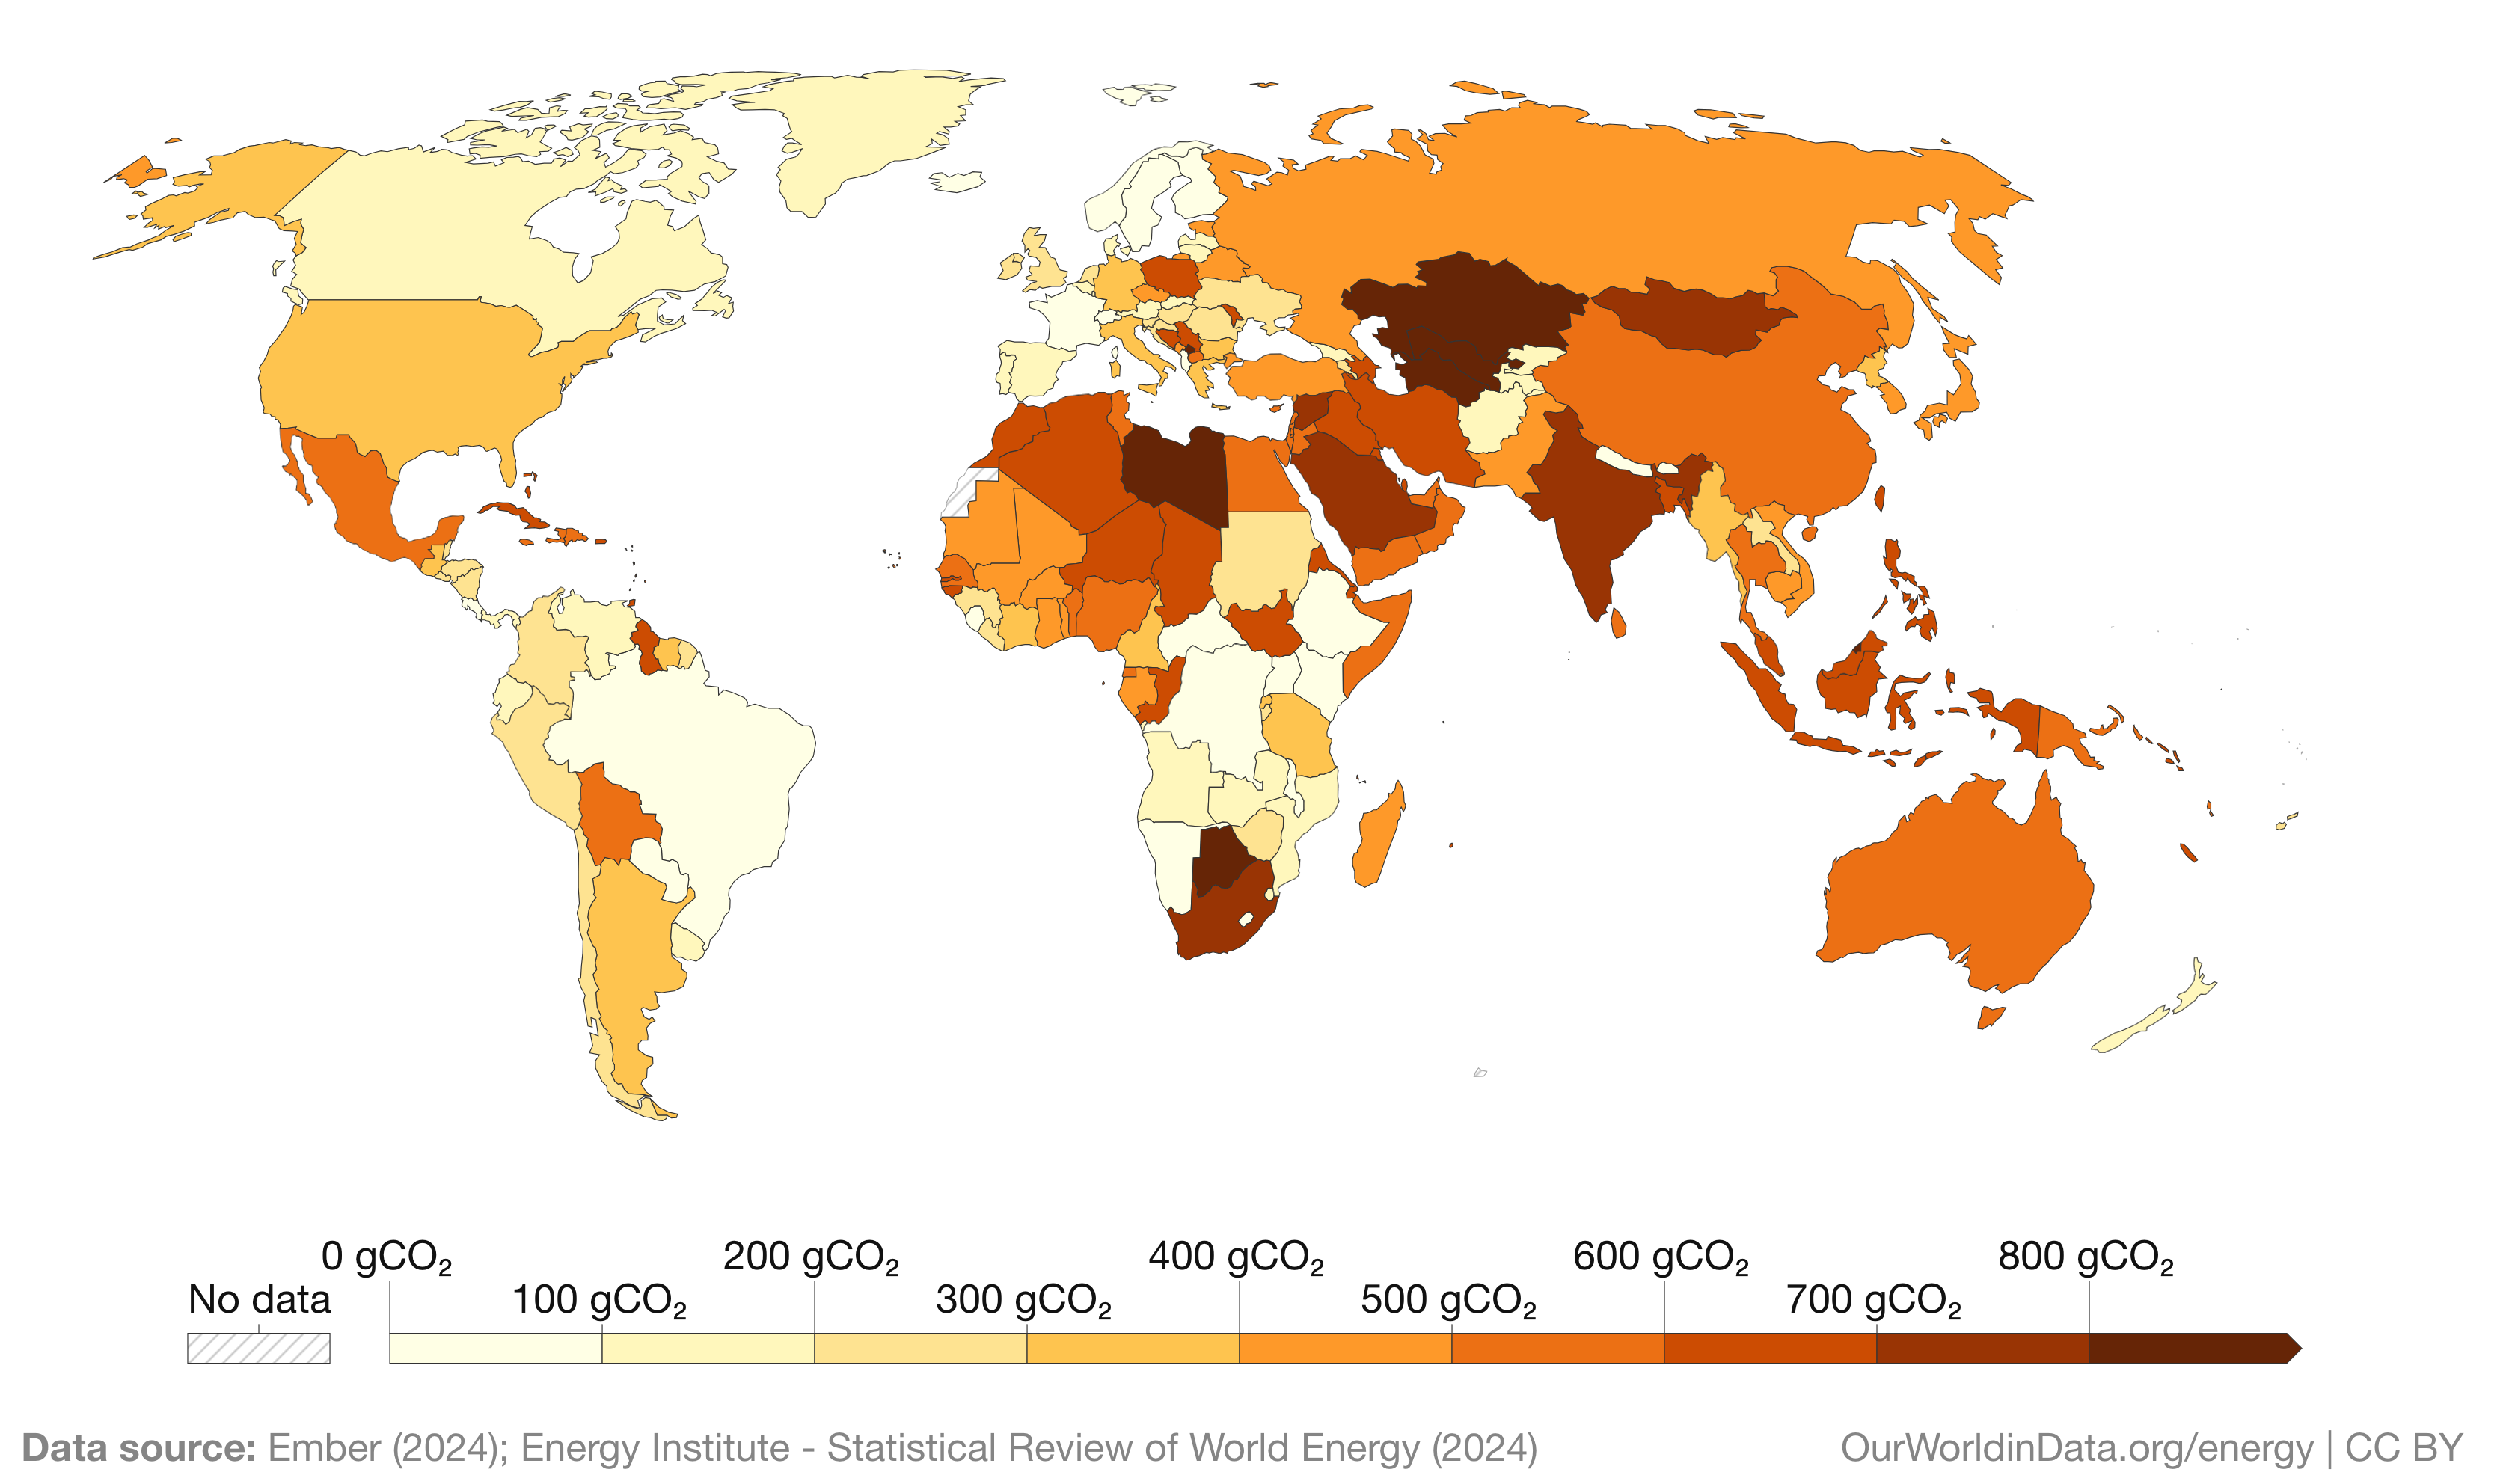
\includegraphics[width=\linewidth]{imgs/carbon-intensity-electricity.png}
    \caption{Carbon intensity of electricity generation, 2023. Source: \cite{ember2024carbonintensity}}
    \label{fig:carbon_intensity}
\end{figure}

By integrating real-time hardware usage monitoring with location-based carbon intensity data, CodeCarbon enables researchers 
and practitioners to quantify the environmental impact of their computations. This information can help guide decision-making, 
such as optimizing code efficiency, choosing lower-carbon data centers, or scheduling workloads during periods of higher renewable 
energy availability.

\section{Extending HADA with CodeCarbon}

\subsection{Energy Management Algorithms}

The first step in extending HADA to incorporate Carbon Intensity is to construct a dataset that includes carbon footprint data from 
algorithm execution. This requires integrating \textbf{CodeCarbon} into the computational workflow used for running algorithms. 

For this study, we analyzed two algorithms: \textbf{ANTICIPATE} and \textbf{CONTINGENCY}, originally introduced in 
\cite{ijcai2019p150, 10.1007/978-3-319-93031-2_8} and previously used in the HADA framework paper \cite{DEFILIPPO2022109199}. 
These algorithms belong to the domain of \textbf{Energy Management Systems} and are designed to compute the amount of energy 
that must be generated to meet a required load while minimizing the total energy cost over a daily time horizon. Both methods
consider the inherent uncertainty in energy demand and production.

\begin{itemize}
    \item \textbf{ANTICIPATE} is an \textit{online}, scenario-based anticipatory algorithm that adapts dynamically to uncertainty.
    \item \textbf{CONTINGENCY} is a hybrid \textit{offline/online} approach that first constructs (offline) a pool of solutions, 
    which is then used to guide an efficient online decision-making process.
\end{itemize}

Both methods are characterized by a tunable configuration parameter that can be adjusted based on performance constraints, 
particularly execution time and solution quality:
\begin{itemize}
    \item For \textbf{ANTICIPATE}, the configuration parameter is the number of considered \textit{scenarios} (\verb|nScenarios|).
    \item For \textbf{CONTINGENCY}, it is the number of \textit{traces} (\verb|nTraces|).
\end{itemize}

The goal of HADA is to learn the relationship between this configuration parameter and various performance metrics that characterize 
algorithm efficiency and resource usage. The original dataset used in HADA includes the following attributes:

\begin{itemize}
    \item \verb|nParam|: The configuration parameter of the algorithm (\verb|nScenarios| for ANTICIPATE, \verb|nTraces| for 
    CONTINGENCY).
    \item \verb|time(s)|: Execution time required to find a solution.
    \item \verb|sol(keuro)|: Cost of the obtained solution (expressed in thousand euros), serving as a measure of solution quality.
    \item \verb|memAvg(MB)|: Average memory usage of the algorithm (in MB).
\end{itemize}

\subsection{Incorporating Energy and Carbon Footprint Metrics}

To extend this approach, we integrated additional metrics related to \textbf{energy consumption} and \textbf{carbon footprint}, 
leveraging the capabilities of CodeCarbon. The following attributes were added to the dataset:

\begin{itemize}
    \item \verb|emissions|: Total $\mathsf{CO_2e}$ emissions generated during execution (kg).
    \item \verb|emission_rate|: Rate of $\mathsf{CO_2e}$ emissions per second (kg/s).
    \item \verb|cpu_energy|: Energy consumed by the CPU (kWh).
    \item \verb|ram_energy|: Energy consumed by RAM (kWh).
    \item \verb|tot_energy|: Total energy consumption (kWh), which is the sum of \verb|cpu_energy| and \verb|ram_energy|. If 
    applicable, it also includes GPU energy consumption.
    \item \verb|country| and \verb|region|: Geographic location where the computation took place, used to determine the carbon 
    intensity of electricity.
    \item \verb|cpu_count|: Number of CPU cores used.
\end{itemize}

Additionally, we implemented tracking for the peak memory usage of each execution, which we included in the dataset under the 
attribute:

\begin{itemize}
    \item \verb|memPeak(MB)|: Maximum memory usage (in MB) recorded during execution.
\end{itemize}

By incorporating these additional metrics, HADA can now model not only algorithm efficiency and solution quality but also the 
environmental impact of computational workloads. This enhancement allows for a more comprehensive optimization approach, balancing 
performance requirements with sustainability considerations.

\subsection{Min-Cut/Max-Flow Algorithms}

Following our initial experiments with ANTICIPATE and CONTINGENCY, which were already included in HADA, we sought to extend our 
study to a broader class of algorithms. We selected a set of algorithms used to solve the \textbf{Minimum Cut/Maximum Flow 
(Min-Cut/Max-Flow)} problem in graphs, a fundamental problem in combinatorial optimization with widespread applications in various 
domains, particularly in \textbf{Computer Vision}. 

The Min-Cut/Max-Flow problem involves computing the maximum amount of flow that can be sent from a designated source node to a 
ink node in a flow network, subject to capacity constraints on edges. The \textbf{Max-Flow} problem seeks to maximize the total 
flow, while the \textbf{Min-Cut} problem finds the smallest set of edges that, if removed, would disconnect the source from the sink. 
The Max-Flow problem and the Min-Cut problem are closely related, as stated by the \textbf{Max-Flow Min-Cut Theorem}, which asserts 
that the maximum flow value in a network is equal to the capacity of the minimum cut.

Min-Cut/Max-Flow algorithms are widely used in image segmentation, stereo vision, and other Computer Vision tasks where images are 
represented as graphs, and energy minimization techniques are applied to solve labeling problems. We referred to the work of Jensen 
et al. (2023) \cite{Jensen2023Maxflow}, which provides a comprehensive review of state-of-the-art Min-Cut/Max-Flow algorithms, 
evaluated on a large dataset of Computer Vision problems. 

\subsubsection{Selected Algorithms}

Based on the findings of Jensen et al., we focused on three well-known Min-Cut/Max-Flow algorithms, each representing different 
families of flow-based optimization methods:

\begin{itemize}
    \item \textbf{Boykov-Kolmogorov (BK)}
    \item \textbf{Excess Incremental Breadth First Search (EIBFS)}
    \item \textbf{Hochbaum's Pseudo-Flow (HPF)}
\end{itemize}

According to Jensen et al., Min-Cut/Max-Flow algorithms can be broadly classified into different families based on their approach 
to augmenting paths and flow computation. The \textbf{Boykov-Kolmogorov} (BK) algorithm \cite{bk2004maxflow} belongs to the \textbf{Augmenting Paths 
(AP)} family, which is one of the oldest methods for solving the Max-Flow problem. This family dates back to the classical 
\textbf{Ford-Fulkerson Algorithm} \cite{ford1956maxflow}, which introduced the concept of augmenting paths to iteratively 
increase the flow. BK extends this approach by introducing heuristic techniques to improve efficiency, making it particularly 
effective for Computer Vision applications.

On the other hand, \textbf{Excess Incremental Breadth First Search (EIBFS)} \cite{goldberg2015faster} and \textbf{Hochbaum’s 
Pseudo-Flow (HPF)} \cite{hochbaum2008pseudoflow} belong to the \textbf{Pseudoflow} family, which differs from augmenting path 
methods in the way it manages flow excess. These algorithms prioritize maintaining a valid preflow at all times and use alternative 
strategies to push flow across the network, often improving efficiency in large-scale instances. 

The main differences between these algorithm families lie in the order in which they traverse nodes while searching for augmenting 
paths and in their mechanisms for pushing flow along paths in the graph.

\subsubsection{Algorithm Variants Considered}

Unlike ANTICIPATE and CONTINGENCY, which have explicit tunable configuration parameters, these Min-Cut/Max-Flow algorithms can 
be implemented with different optimizations \cite{Jensen2023Maxflow}. We treated the specific implementation variant of each algorithm as a configuration 
parameter and considered the following versions:

\begin{itemize}
    \item \textbf{Boykov-Kolmogorov (BK) Variants:}
    \begin{itemize}
        \item \textbf{BK}: The reference implementation.
        \item \textbf{MBK}: An optimized version by Jensen et al., using indices instead of pointers to reduce memory footprint.
        \item \textbf{MBK-R}: A second optimized version that reorders arcs to ensure that all outgoing edges from a node are 
        stored contiguously in memory.
    \end{itemize}
    \item \textbf{Excess Incremental Breadth First Search (EIBFS) Variants:}
    \begin{itemize}
        \item \textbf{EIBFS}: A slightly modified version of the original EIBFS algorithm.
        \item \textbf{EIBFS-I}: A version that replaces pointers with indices to improve memory locality.
        \item \textbf{EIBFS-I-NR}: A version similar to EIBFS-I but without arc reordering.
    \end{itemize}
    \item \textbf{Hochbaum’s Pseudo-Flow (HPF) Variants:}
    \begin{itemize}
        \item \textbf{HPF-H-F}: Highest-label variant using FIFO buckets.
        \item \textbf{HPF-H-L}: Highest-label variant using LIFO buckets.
        \item \textbf{HPF-L-F}: Lowest-label variant using FIFO buckets.
        \item \textbf{HPF-L-L}: Lowest-label variant using LIFO buckets.
    \end{itemize}
\end{itemize}

\subsubsection{Energy and Carbon Footprint Monitoring}

Jensen et al. provided scripts to evaluate the runtime performance of these algorithms, measuring both initialization time and 
execution time. To extend this analysis with energy consumption and carbon footprint tracking, we modified their experimental 
setup by integrating \textbf{CodeCarbon}. 

Since the original implementations are written in C++, we wrapped the algorithm scripts with a Python interface to facilitate 
real-time monitoring. This wrapper was designed to:
\begin{itemize}
    \item Track memory usage throughout execution.
    \item Use CodeCarbon to measure CPU and RAM energy consumption.
    \item Record $\mathsf{CO_2e}$ emissions based on the energy consumption and Carbon Intensity of the execution environment.
\end{itemize}

Unlike the experiments with ANTICIPATE and CONTINGENCY, where solution quality was a critical performance metric, here we focus 
solely on computational efficiency. The primary metrics of interest for this study are execution time, memory consumption, energy 
consumption, and environmental impact. By incorporating these Min-Cut/Max-Flow algorithms into HADA, we aim to explore 
energy-efficient graph-based optimization techniques and further refine our approach to sustainable AI computation.

\chapter{Experimental Analysis}

\section{Benchmarking on Different Hardware Platforms}

For the benchmark phase, we opted for running the algorithms on different Hardware Platforms, in order to better capture the differences in performance
when changing the machine on which the algorithm is executed:

Experiments were conducted on:
\begin{itemize}
\item \verb|mbp19|: A Laptopr running MacOS Ventura 13.6.7 with:
    \begin{itemize}
        \item 1,4 GHz Quad-Core Intel Core i5;
        \item 8 GB 2133 MHz LPDDR3;
    \end{itemize}
\item \verb|PC|: A PC with Ubuntu 22.0.4 LTS
\item \verb|leonardo| An HPC infrastructure, i.e. Leonardo hosted by CINECA. It has a total of 4992 computing nodes organized in two partitions, the Booster partition and the Data Centric General Purpose (DCGP) partition. For running the benchmark phase we used the booster partition, which has the following specifics:
    \begin{itemize}
        \item 8×64 GB DDR4 3200 MHz (512 GB)
        \item single socket 32-core Intel Xeon Platinum 8358 CPU, 2.60GHz (Ice Lake) (110592 cores).
        \item 4x NVIDIA custom Ampere A100 GPU 64GB HBM2e, NVLink 3.0 (200GB/s)
    \end{itemize}
\end{itemize}

ANTICIPATE and CONTINGENCY were executed on 30 instances which were sampled with a statistical model with a Gaussian distribution \cite{DEFILIPPO2022109199}.
On each instance, each algorithm was executed with parameter (i.e. number of traces or scenarios) values ranging from 1 to 100. For ANTICIPATE and CONTINGENCY we
used only \verb|mbp19| and \verb|leonardo|. Thus in the end we obtained a dataset with a total of $30 \times 100 \times 2 \times 2 = 12,000$ entries. 

To generate a benchmark dataset for the Min-Cut/Max-Flow algorithms, we relied on the dataset provided by Jensen et al. (2023) \cite{Jensen2023Maxflow}. This is an extensive collection of instances
of Min-Cut/Max-Flow problems in the Computer Vision field. The authors also provided the implementations of the algorithms that were used to generate our benchmark data.
Since they are implemented in C++ (BK and EIBFS) and C (HPF), we faced the problem of how to track the energy consumption and thus the emissions of such code. Apparently,
there are not much tool available to monitor the emissions of C code. % TODO: expand this in the RELATED WORK SECTION.
We opted for using a python wrapper script, that runs the C++/C scripts implementing the algorithms and uses CodeCarbon to track the energy consumption of the script execution.
For reasons due to lacking support on MacOS, i was not able to compile the BK and EIBFS implementation on mbp19. Instead, i have managed to restore an old PC i had at home 
with a light distribution of Ubuntu to run some of these scripts. 
It is important to point out that we did not executed the selected algorithms on the whole dataset, since some of the problem instances were very big, sometimes exceeding the available memory,
we just ran a subset of them - even if it was possible to create a swap partition big enough to accomodate bigger instances, the monitoring tools available just record the 
used RAM, so the estimate of the memory usage would be downsized in such cases. Also, due to the large number of instances, running a benchmark phase on all of them would have
been way too time consuming. 

\subsection{ANTICIPATE and CONTINGENCY}

% BOX PLOTS

\begin{figure}[h!]
    \centering
    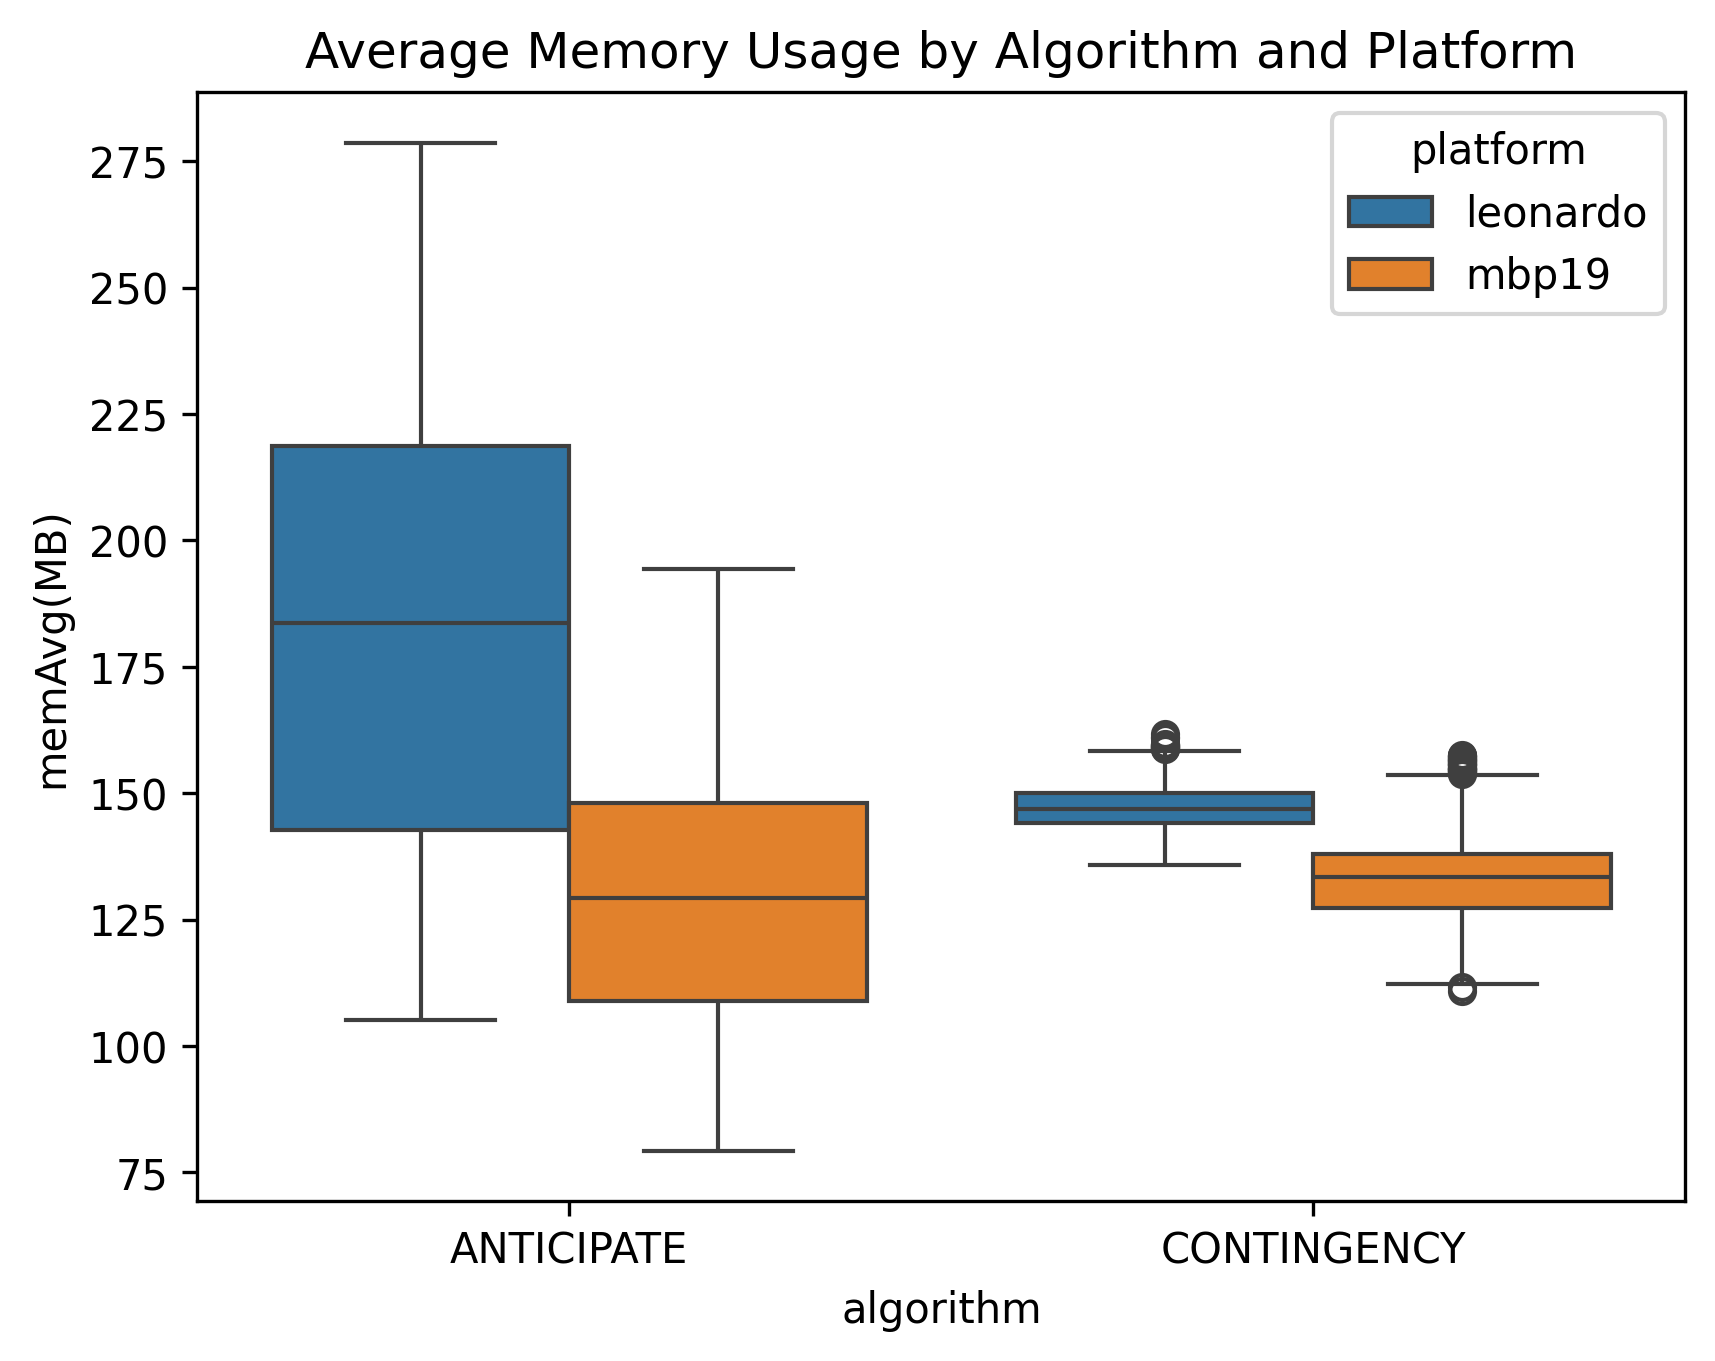
\includegraphics[width=0.8\textwidth]{imgs/avg_mem_usage.png}
    \caption{Average memory usage of ANTICIPATE and CONTINGENCY divided by platform}
    \label{fig:ant_cont_avg_mem_usage}
\end{figure}

\begin{figure}[h!]
    \centering
    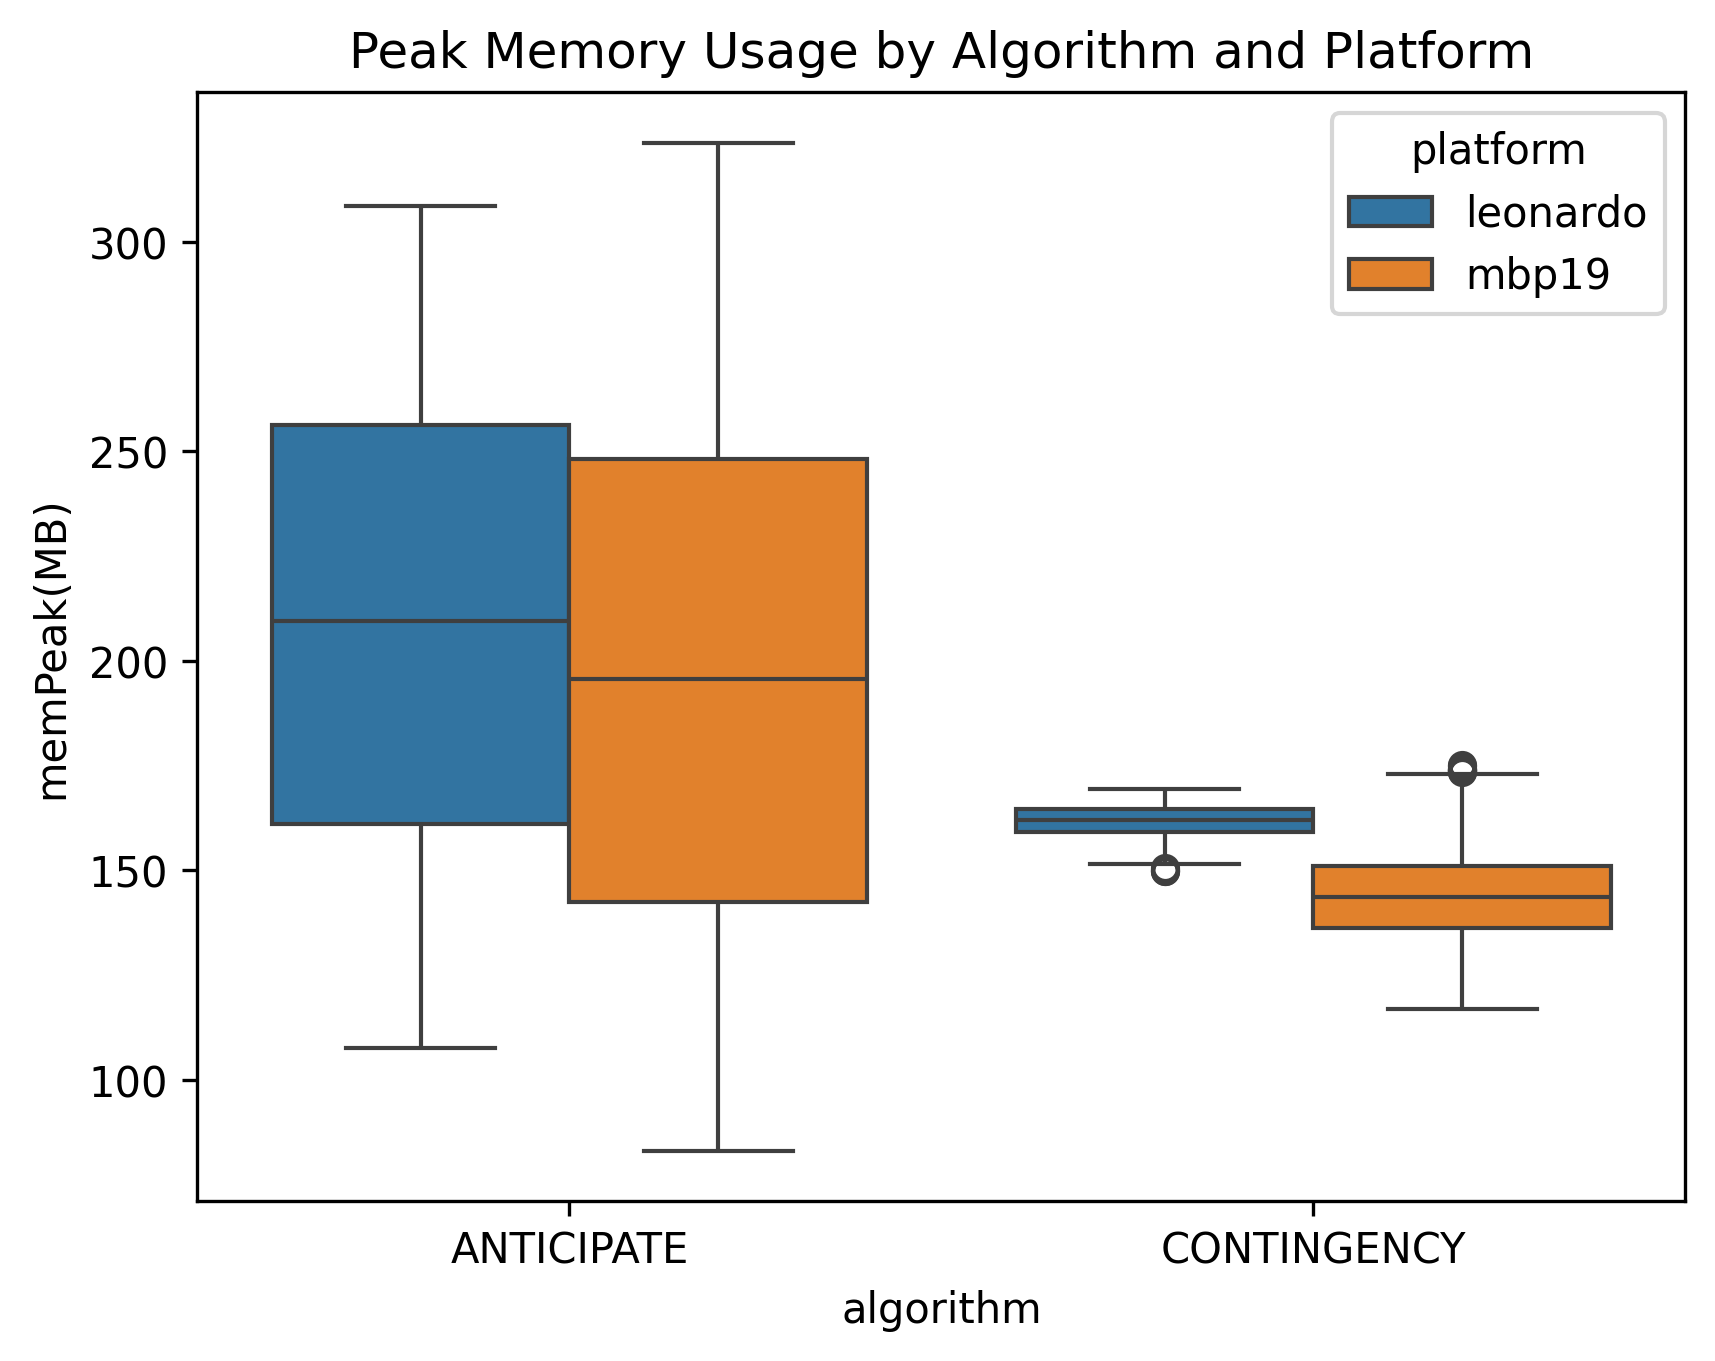
\includegraphics[width=0.8\textwidth]{imgs/peak_mem_usage.png}
    \caption{Peak memory usage of ANTICIPATE and CONTINGENCY divided by platform}
    \label{fig:ant_cont_peak_mem_usage}
\end{figure}

\begin{figure}[h!]
    \centering
    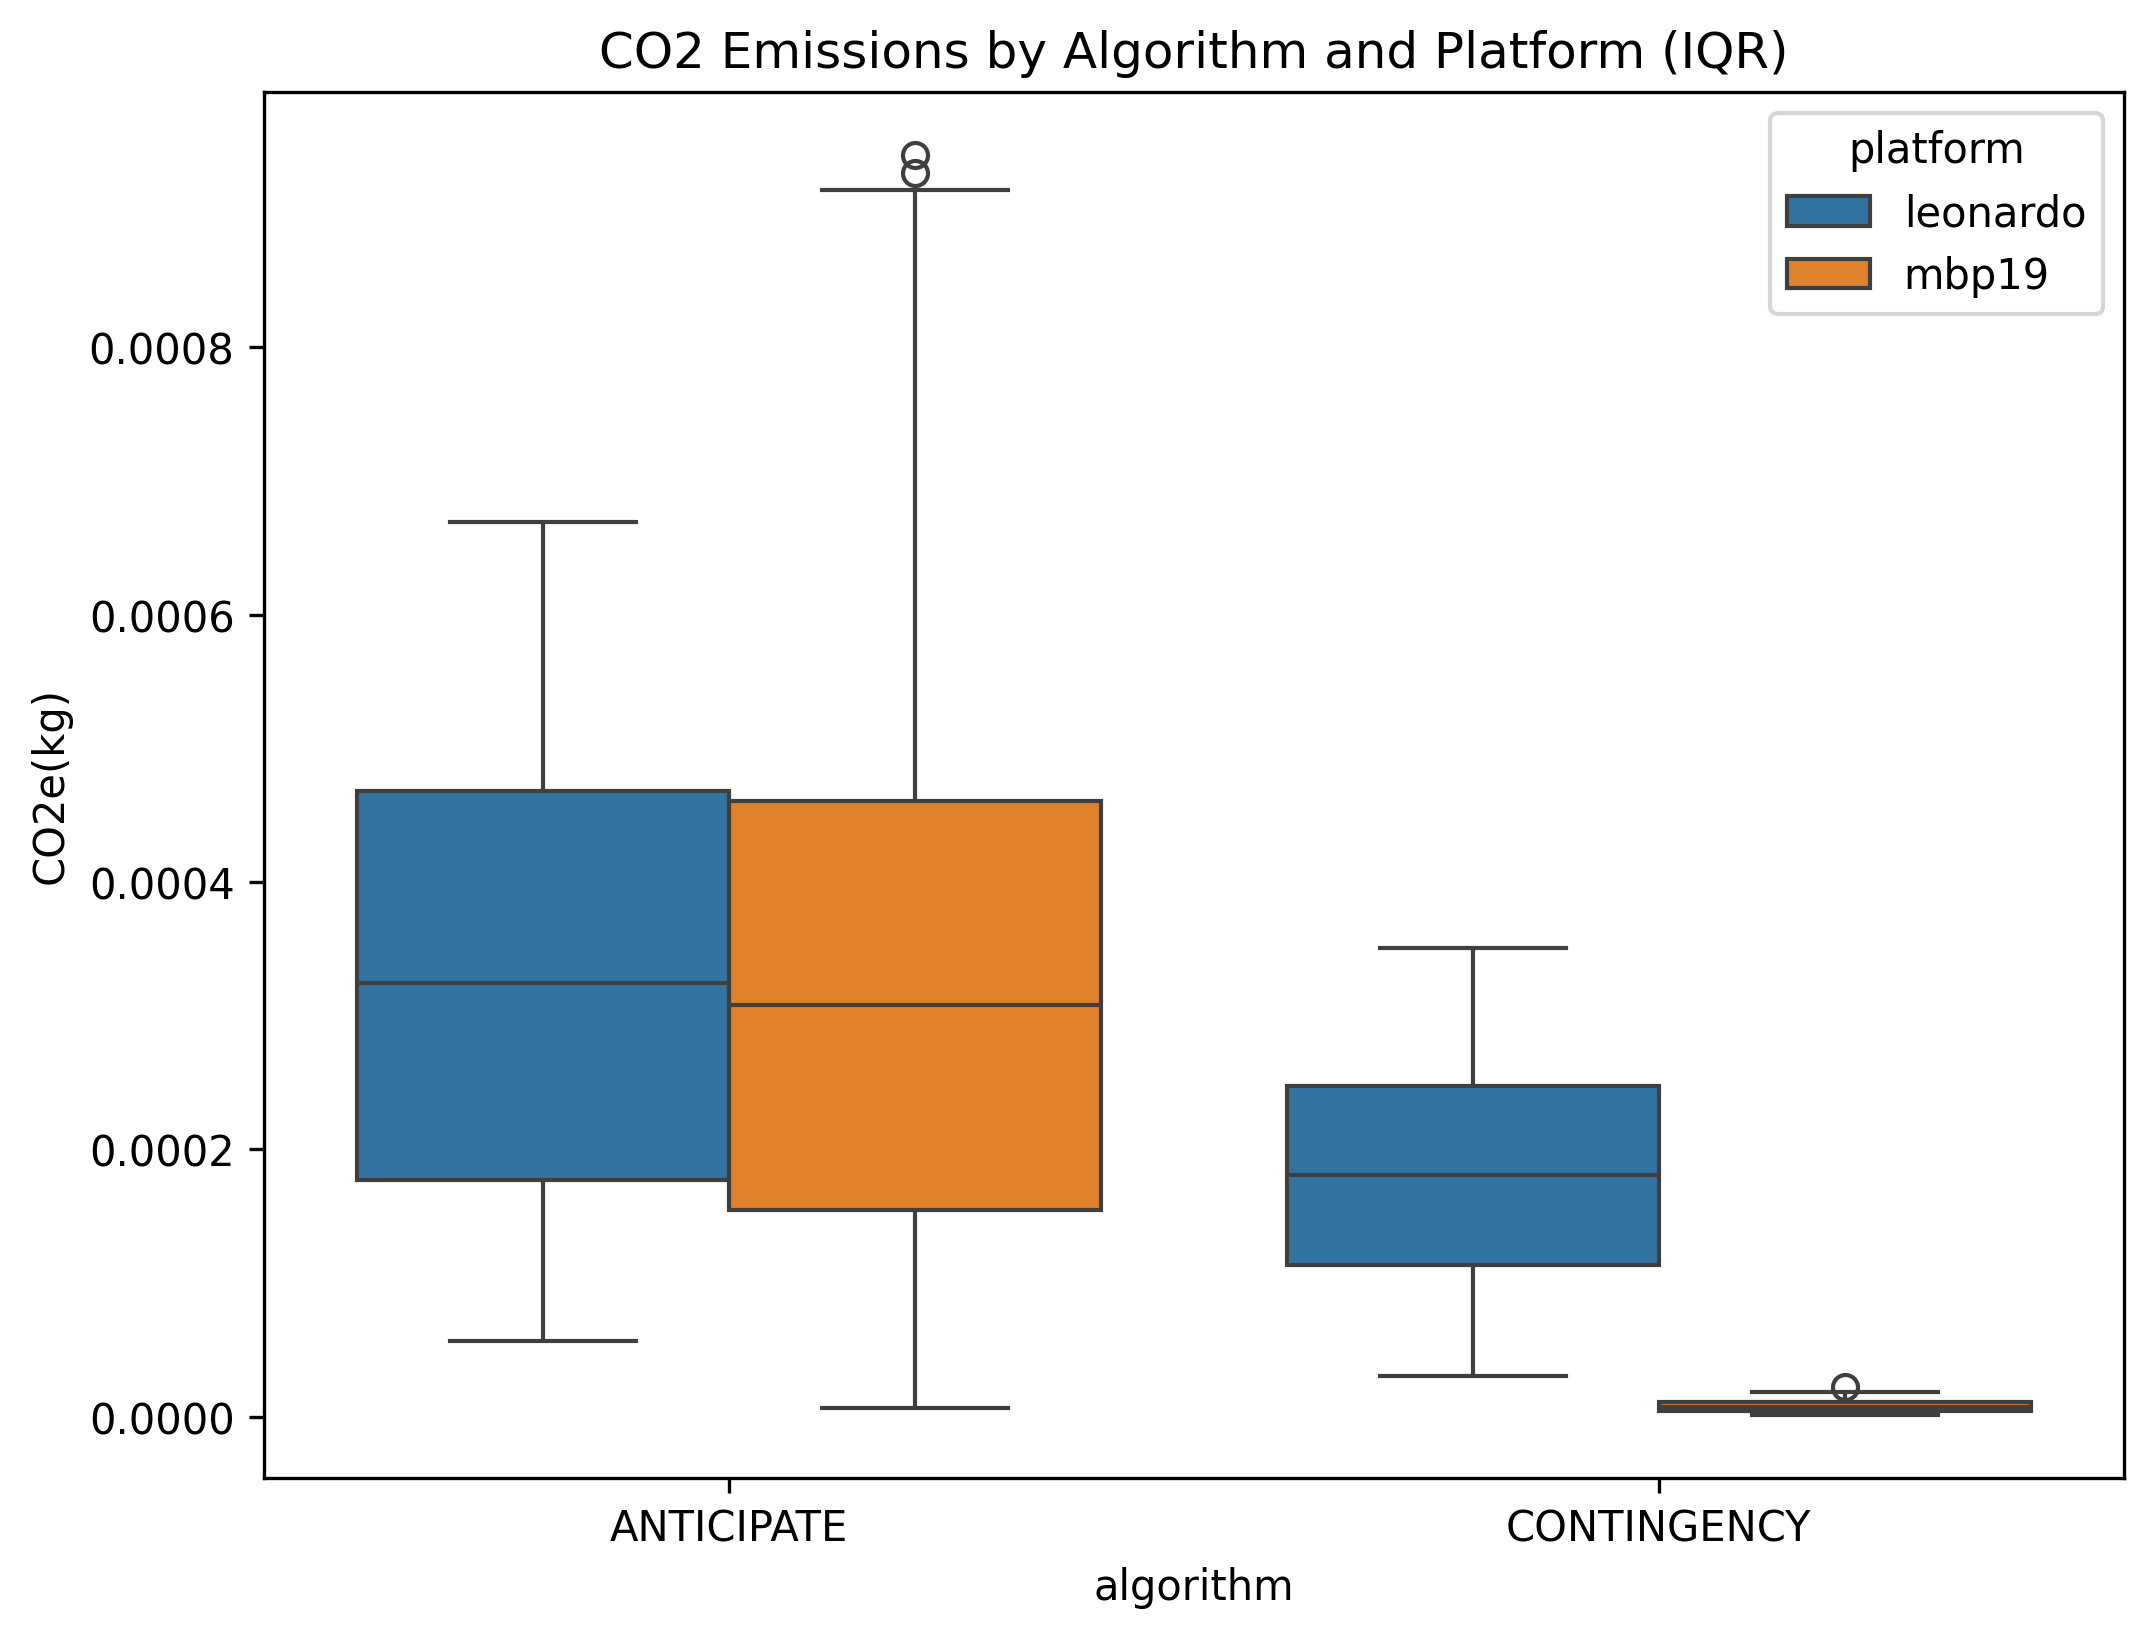
\includegraphics[width=0.8\textwidth]{imgs/CO2_emissions_no_outliers.png}
    \caption{CO2 emissions for ANTICIPATE and CONGINGENCY ordered by platform}
    \label{fig:ant_cont_co2_emissions}
\end{figure}

\begin{figure}[h!]
    \centering
    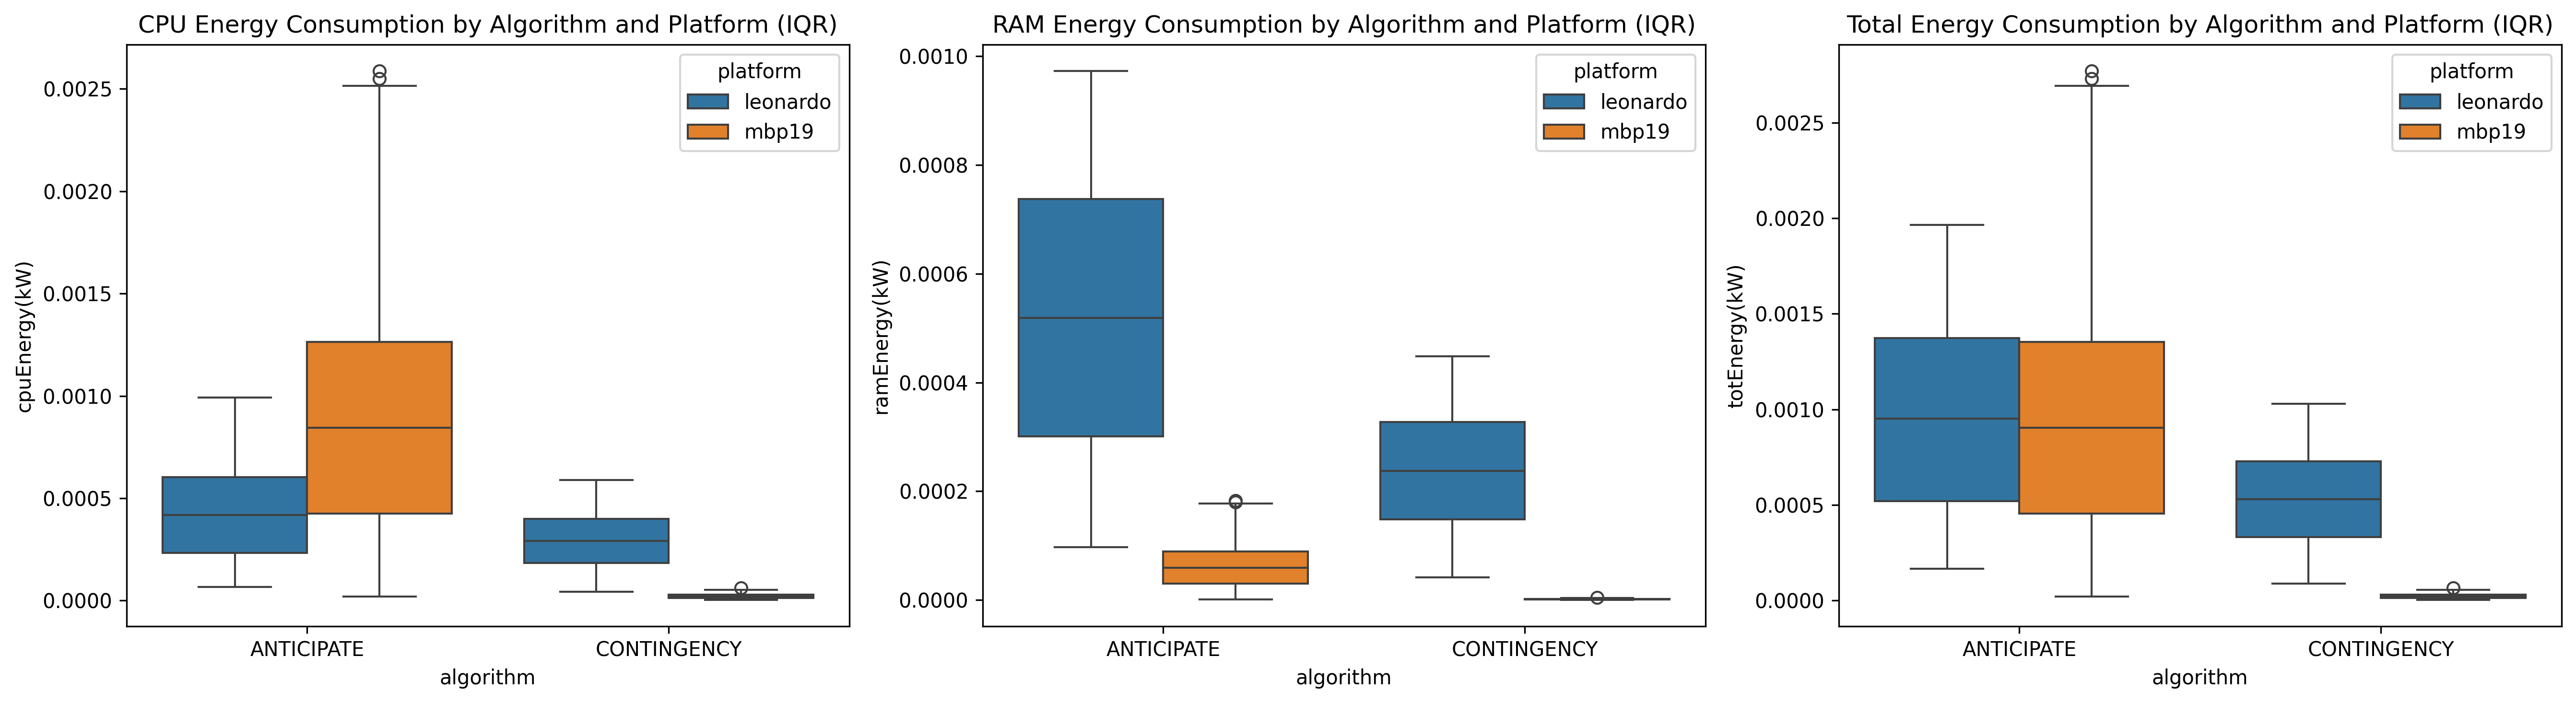
\includegraphics[width=0.8\textwidth]{imgs/energy_consumption_no_outliers.png}
    \caption{Energy Consumption data for ANTICIPATE and CONTINGENCY}
    \label{fig:ant_cont_energy}
\end{figure}

% CORRELATION MATRICES

\begin{figure}[h!]
    \centering
    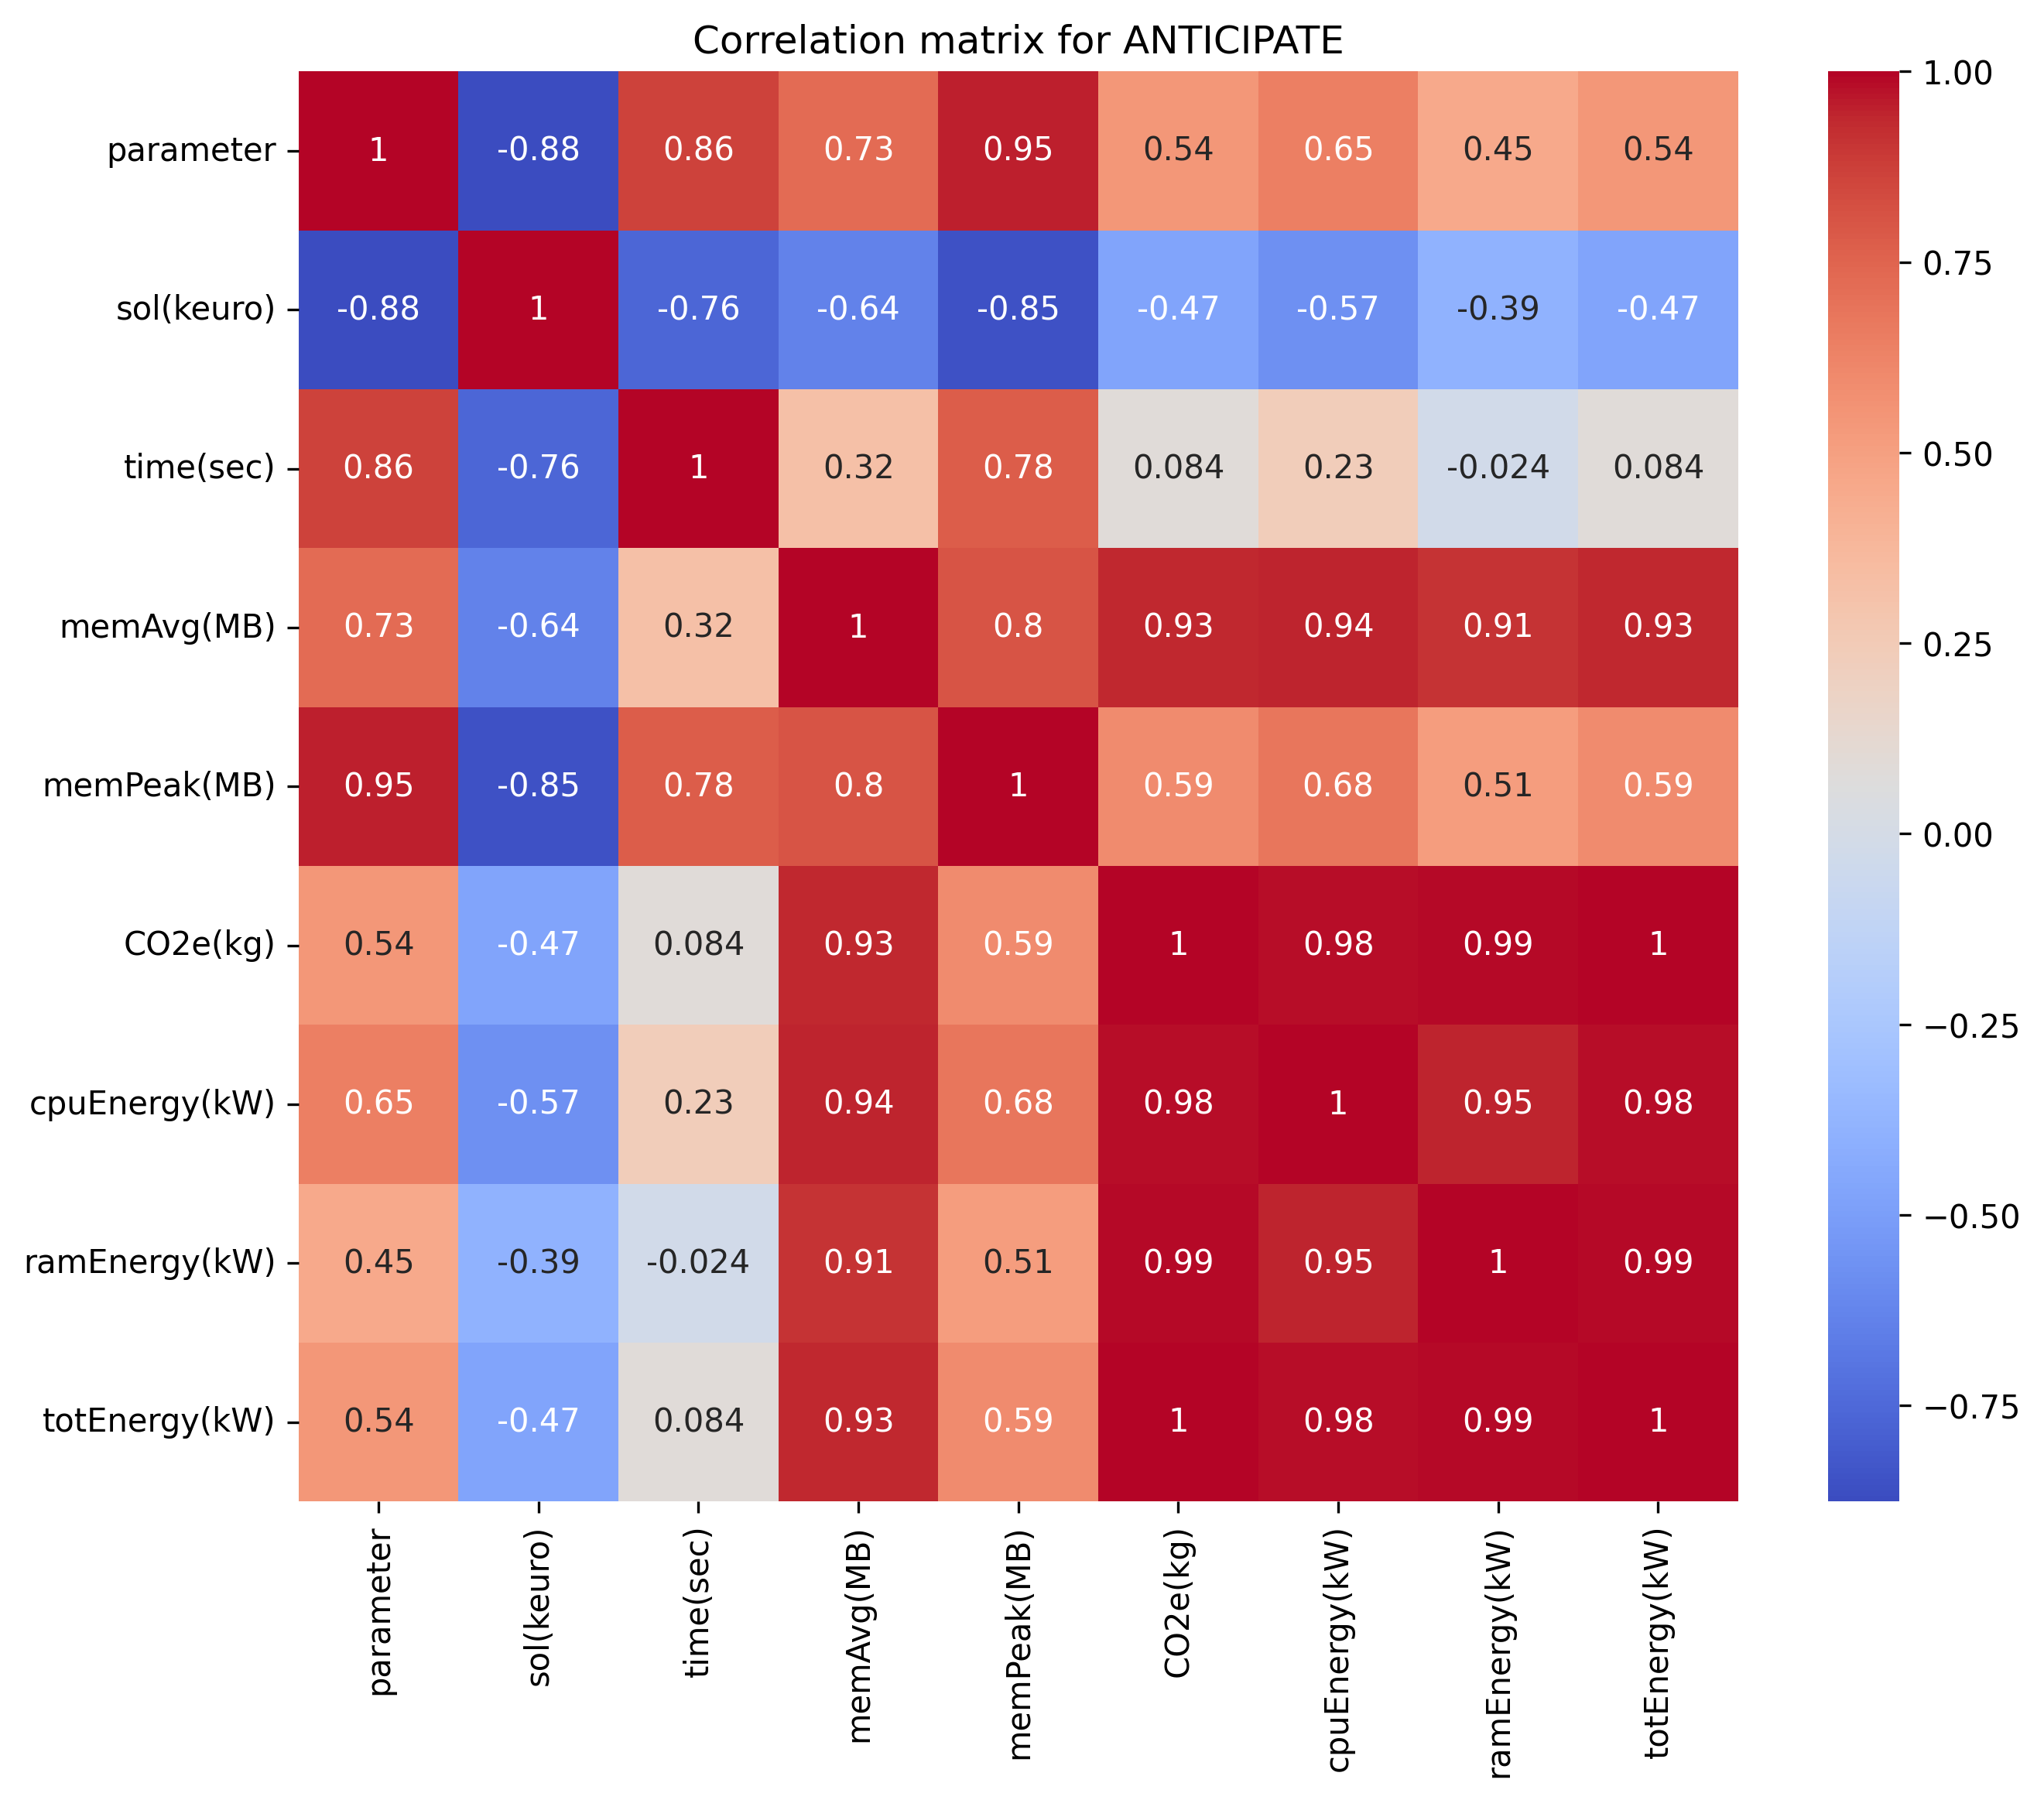
\includegraphics[width=0.8\textwidth]{imgs/ant_corr_mat.png}
    \caption{Correlation matrix for ANTICIPATE}
    \label{fig:ant_corr_mat}
\end{figure}

\begin{figure}[h!]
    \centering
    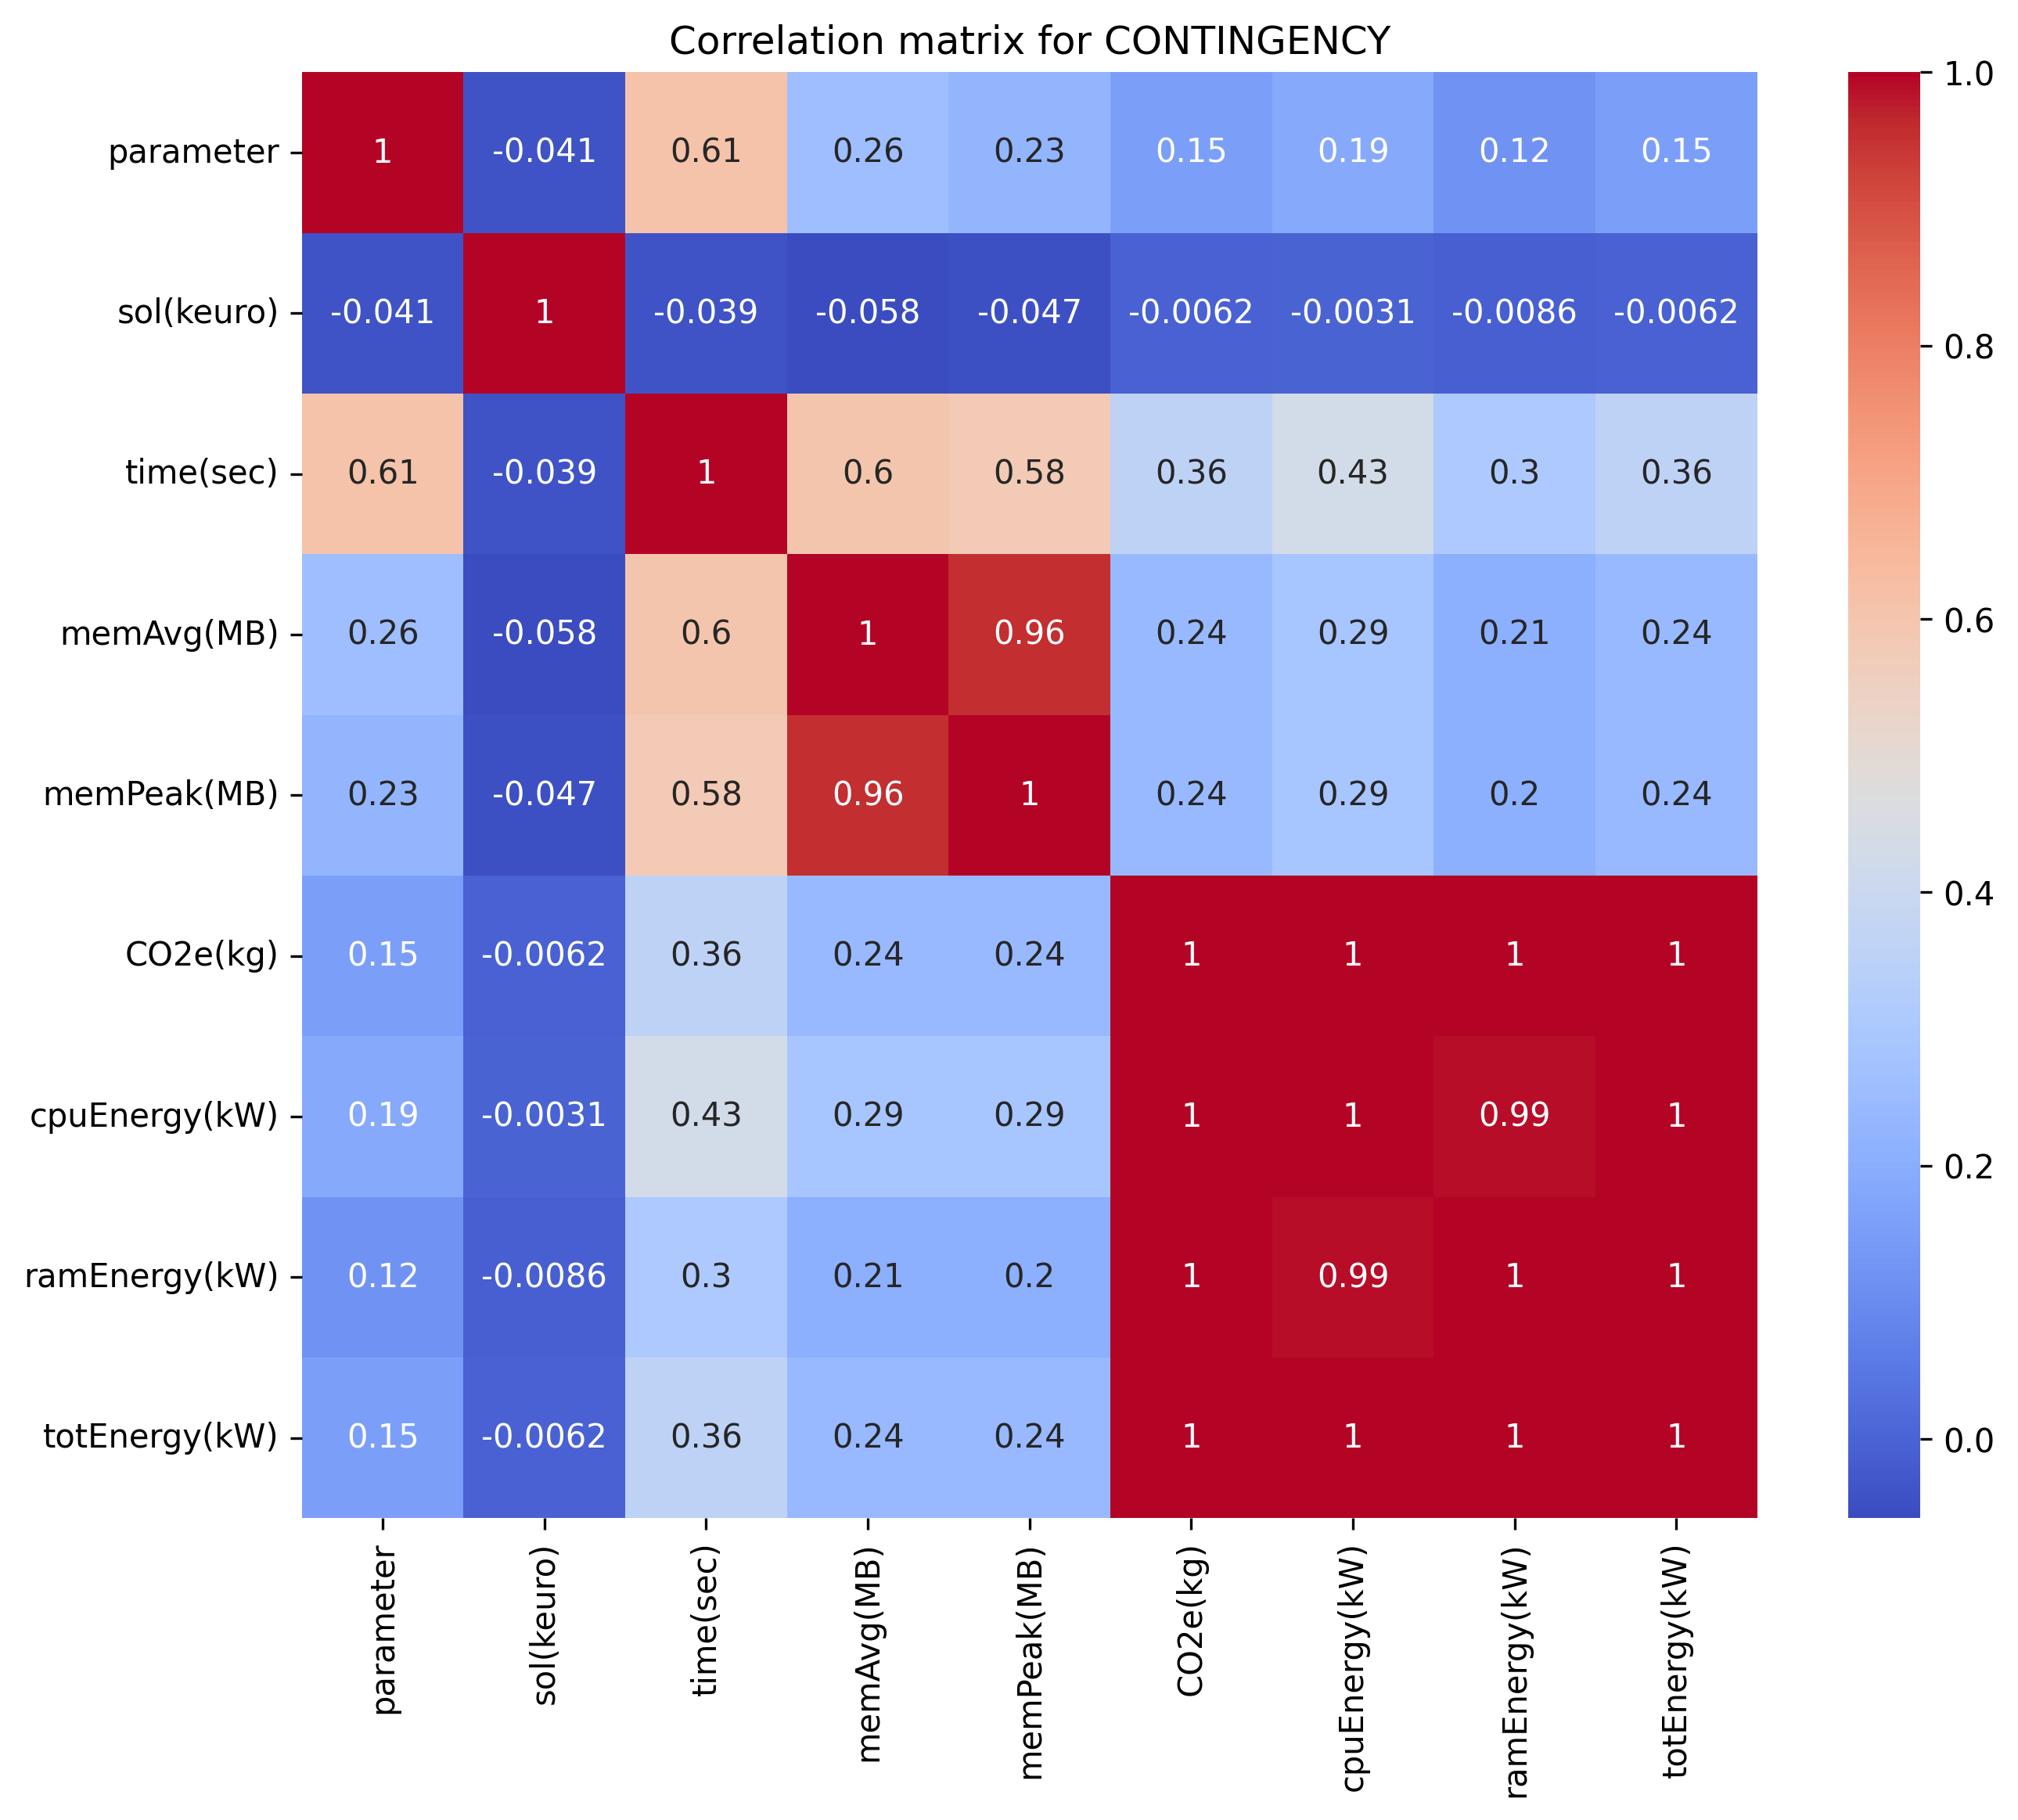
\includegraphics[width=0.8\textwidth]{imgs/cont_corr_mat.png}
    \caption{Correlation matrix for CONTINGENCY}
    \label{fig:cont_corr_mat}
\end{figure}

Here we can see some results given by the HADA framework tested on the updated dataset for ANTICIPATE and CONTINGENCY. \ref{tab:anticipate_results}
presents the results of optimising any target without any constraints for ANTICIPATE. We can notice how, for most metrics keeping the number of scenarios
as low as possible is the best choice, while increasing them brings the solution cost down.

\begin{table}[h!]
    \centering
    \begin{tabular}{|c|ccc|}
        \hline
        \multicolumn{1}{|c|}{Objective} & \multicolumn{3}{c|}{Solution} \\
        \hline
        Target & $n^P$ & HW & Value \\
        \hline
        CO2e (kg) & 1 & mbp19 & $7.23 \times 10^{-6}$ \\
        Cost (€) & 97 & mbp19 & $267.39k$ \\
        Time (s)& 1 & mbp19 & $1.24$ \\
        Avg. Memory (MB) & 1 & mbp19 & $81.47$ \\
        Peak Memory (MB) & 2 & mpb19 & $92.19$ \\
        Energy (kW) & 1 & mbp19 & $2.12$ \\
        \hline
    \end{tabular}
    \caption{Minimum values for each target for the ANTICIPATE algorithm}
    \label{tab:anticipate_min_targets}
\end{table}

\begin{table}[h!]
    \centering
    \begin{tabular}{|c|ccc|}
        \hline
        \multicolumn{1}{|c|}{Objective} & \multicolumn{3}{c|}{Solution} \\
        \hline
        Target & $n^P$ & HW & Value \\
        \hline
        CO2e (kg) & 2 & mbp19 & $1.28 \times 10^{6}$ \\
        Cost (€) & 90 & mbp19 & $314.11k$ \\
        Time (s)& 1 & mbp19 & $5.16$ \\
        Avg. Memory (MB) & 1 & mbp19 & $117.66$ \\
        Peak Memory (MB) & 2 & mbp19 & $130.58$ \\
        Energy (kW) & 2 & mbp19 & $3.77 \times 10^{-6}$ \\
        \hline
    \end{tabular}
    \caption{Minimum values for each target for the CONTINGENCY algorithm}
    \label{tab:contingency_min_targets}
\end{table}

As we can see in \ref{fig:ant_corr_mat}, \verb|totEnergy| has a correlation of $1$ with CO2e, meaning they are perfectly proportional to each other. This reflects the fact that Carbon Emissions,
as measured by CodeCarbon, depends by two factors, i.e. the energy consumed by running the algorithm and the Carbon Intensity. Since we executed all the experiments in the same
country, the Carbon Intensity over the whole dataset is fixed, meaning that the only factor influencing the CO2e emissions is the energy consumed, while the Carbon Intensity
is just a scaling factor. Indeed, \verb|totEnergy| and \verb|CO2e| both the same correlation values with the other variables. Also, as we could expect, the correlation
of \verb|CO2e| with \verb|cpuEnergy| and \verb|ramEnergy| is also pretty high, being of $0.98$ and $0.99$ respectively, and that reflects the fact that actually the total energy consumption is
nothing but the sum of \verb|cpuEnergy| and \verb|ramEnergy|. Then, as one may point out, we could just remove the energy consumption values from the dataset, and just keep the emissions.
However, the energy consumption values can be scaled by different Carbon Intensity values, giving the possibility of evaluating the impact of changing the location of the computations, as we will see later on.
Then, we can see that the average memory consumption is the variable with the highest correlation with the carbon emissions except for energy consumption, with a value of $0.93$. Then, we can see
that for ANTICIPATE the emissions are also influenced a bit by the value of the parameter ($0.65$) and the Solution Cost ($-0.57$). We could then perform some tests on ANTICIPATE with HADA
to asses the impact of constraints on memory and solution quality.

\begin{table}[h!]
    \centering
    \begin{tabular}{|cc|ccccc|}
        \hline
        \multicolumn{2}{|c|}{Bounds} & \multicolumn{5}{c|}{Solution} \\
        \hline
        Memory & Cost & $n^P$ & HW & CO2e & Memory & Cost \\
        \hline
        no & no & 1 & mbp19 & $7.23 \times 10^{-6}$ & - & - \\
        80 & no & none & none & none & none & none \\
        no & $100k$ & none & none & none & none & none \\
        100 & $300k$ & none & none & none & none & none \\
        150 & $300k$ & 64 & mbp19 & $3.75 \times 10^{-4}$ & $141.53$ & $299.46k$ \\
        170 & $270k$ & 97 & mbp19 & $5.70 \times 10^{-4}$ & $169.85$ & $267.39k$ \\
        170 & $280k$ & 87 & mbp19 & $5.10 \times 10^{-4}$ & $160.12$ & $276.86k$ \\
        300 & $500k$ & 1 & mbp19 & $7.23 \times 10^{-6}$ & $81.47$ & $368.73k$ \\
        \hline
    \end{tabular}
    \caption{Experimental results for the ANTICIPATE algorithm with bounds Memory usage and Solution cost}
    \label{tab:anticipate_results}
\end{table}

In \ref{tab:anticipate_results} we can see some the results of some combination of constraints on Solution cost (which is
expressed €), and Average Memory consumption (expressed in MB), with the objective of minimizing the CO2e 
emissions (in kg). The rows filled with "none" indicates that HADA didn't found a solution satisfying those constraints for the
given algorithm.

For CONTINGENCY, \ref{fig:cont_corr_mat} shows how the variables show very little amount of linear correlation between one another. The strongest relation is between the runtime and the amount of memory consumed
(with a score of $0.60$ for \verb|memAvg| and $0.58$ for \verb|memPeak|). As for the Carbon Footprint, the value that influence it the most is the runtime, with a postivie correlation of $0.47$.
So we will try to test HADA on CONTINGENCY with constraints on the Runtime (expressed in seconds), and the Solution cost.

\begin{table}[h!]
    \centering
    \begin{tabular}{|cc|ccccc|}
        \hline
        \multicolumn{2}{|c|}{Bounds} & \multicolumn{5}{c|}{Solution} \\
        \hline
        Time & Cost & $n^P$ & HW & CO2e & Time & Cost \\
        \hline
        no & no & 2 & mbp19 & $1.29 \times 10^{-6}$ & - & - \\
        no & $350k$ & 4 & mbp19 & $1.53 \times 10^{6}$ & - & $338.23k$ \\
        10 & no & 2 & mbp19 & $1.29 \times 10^{-6}$ & $6.01$ & - \\
        10 & $320k$ & none & none & none & none & none \\
        60 & $350k$ & 4 & mbp19 & $1.29 \times 10^{-6}$ & $7.68$ & $338.23$ \\
        120 & $320k$ & 90 & mbp19 & $1.24 \times 10^{-5}$ & $119.47$ & $314.11k$ \\
        \hline
    \end{tabular}
    \caption{Experimental results for the CONTINGENCY algorithm with bounds on Runtime and Memory usage}
    \label{tab:contingency_results}
\end{table}

\subsection{Min-Cut/Max-Flow Algorithms} 

\begin{figure}[h!]
    \centering
    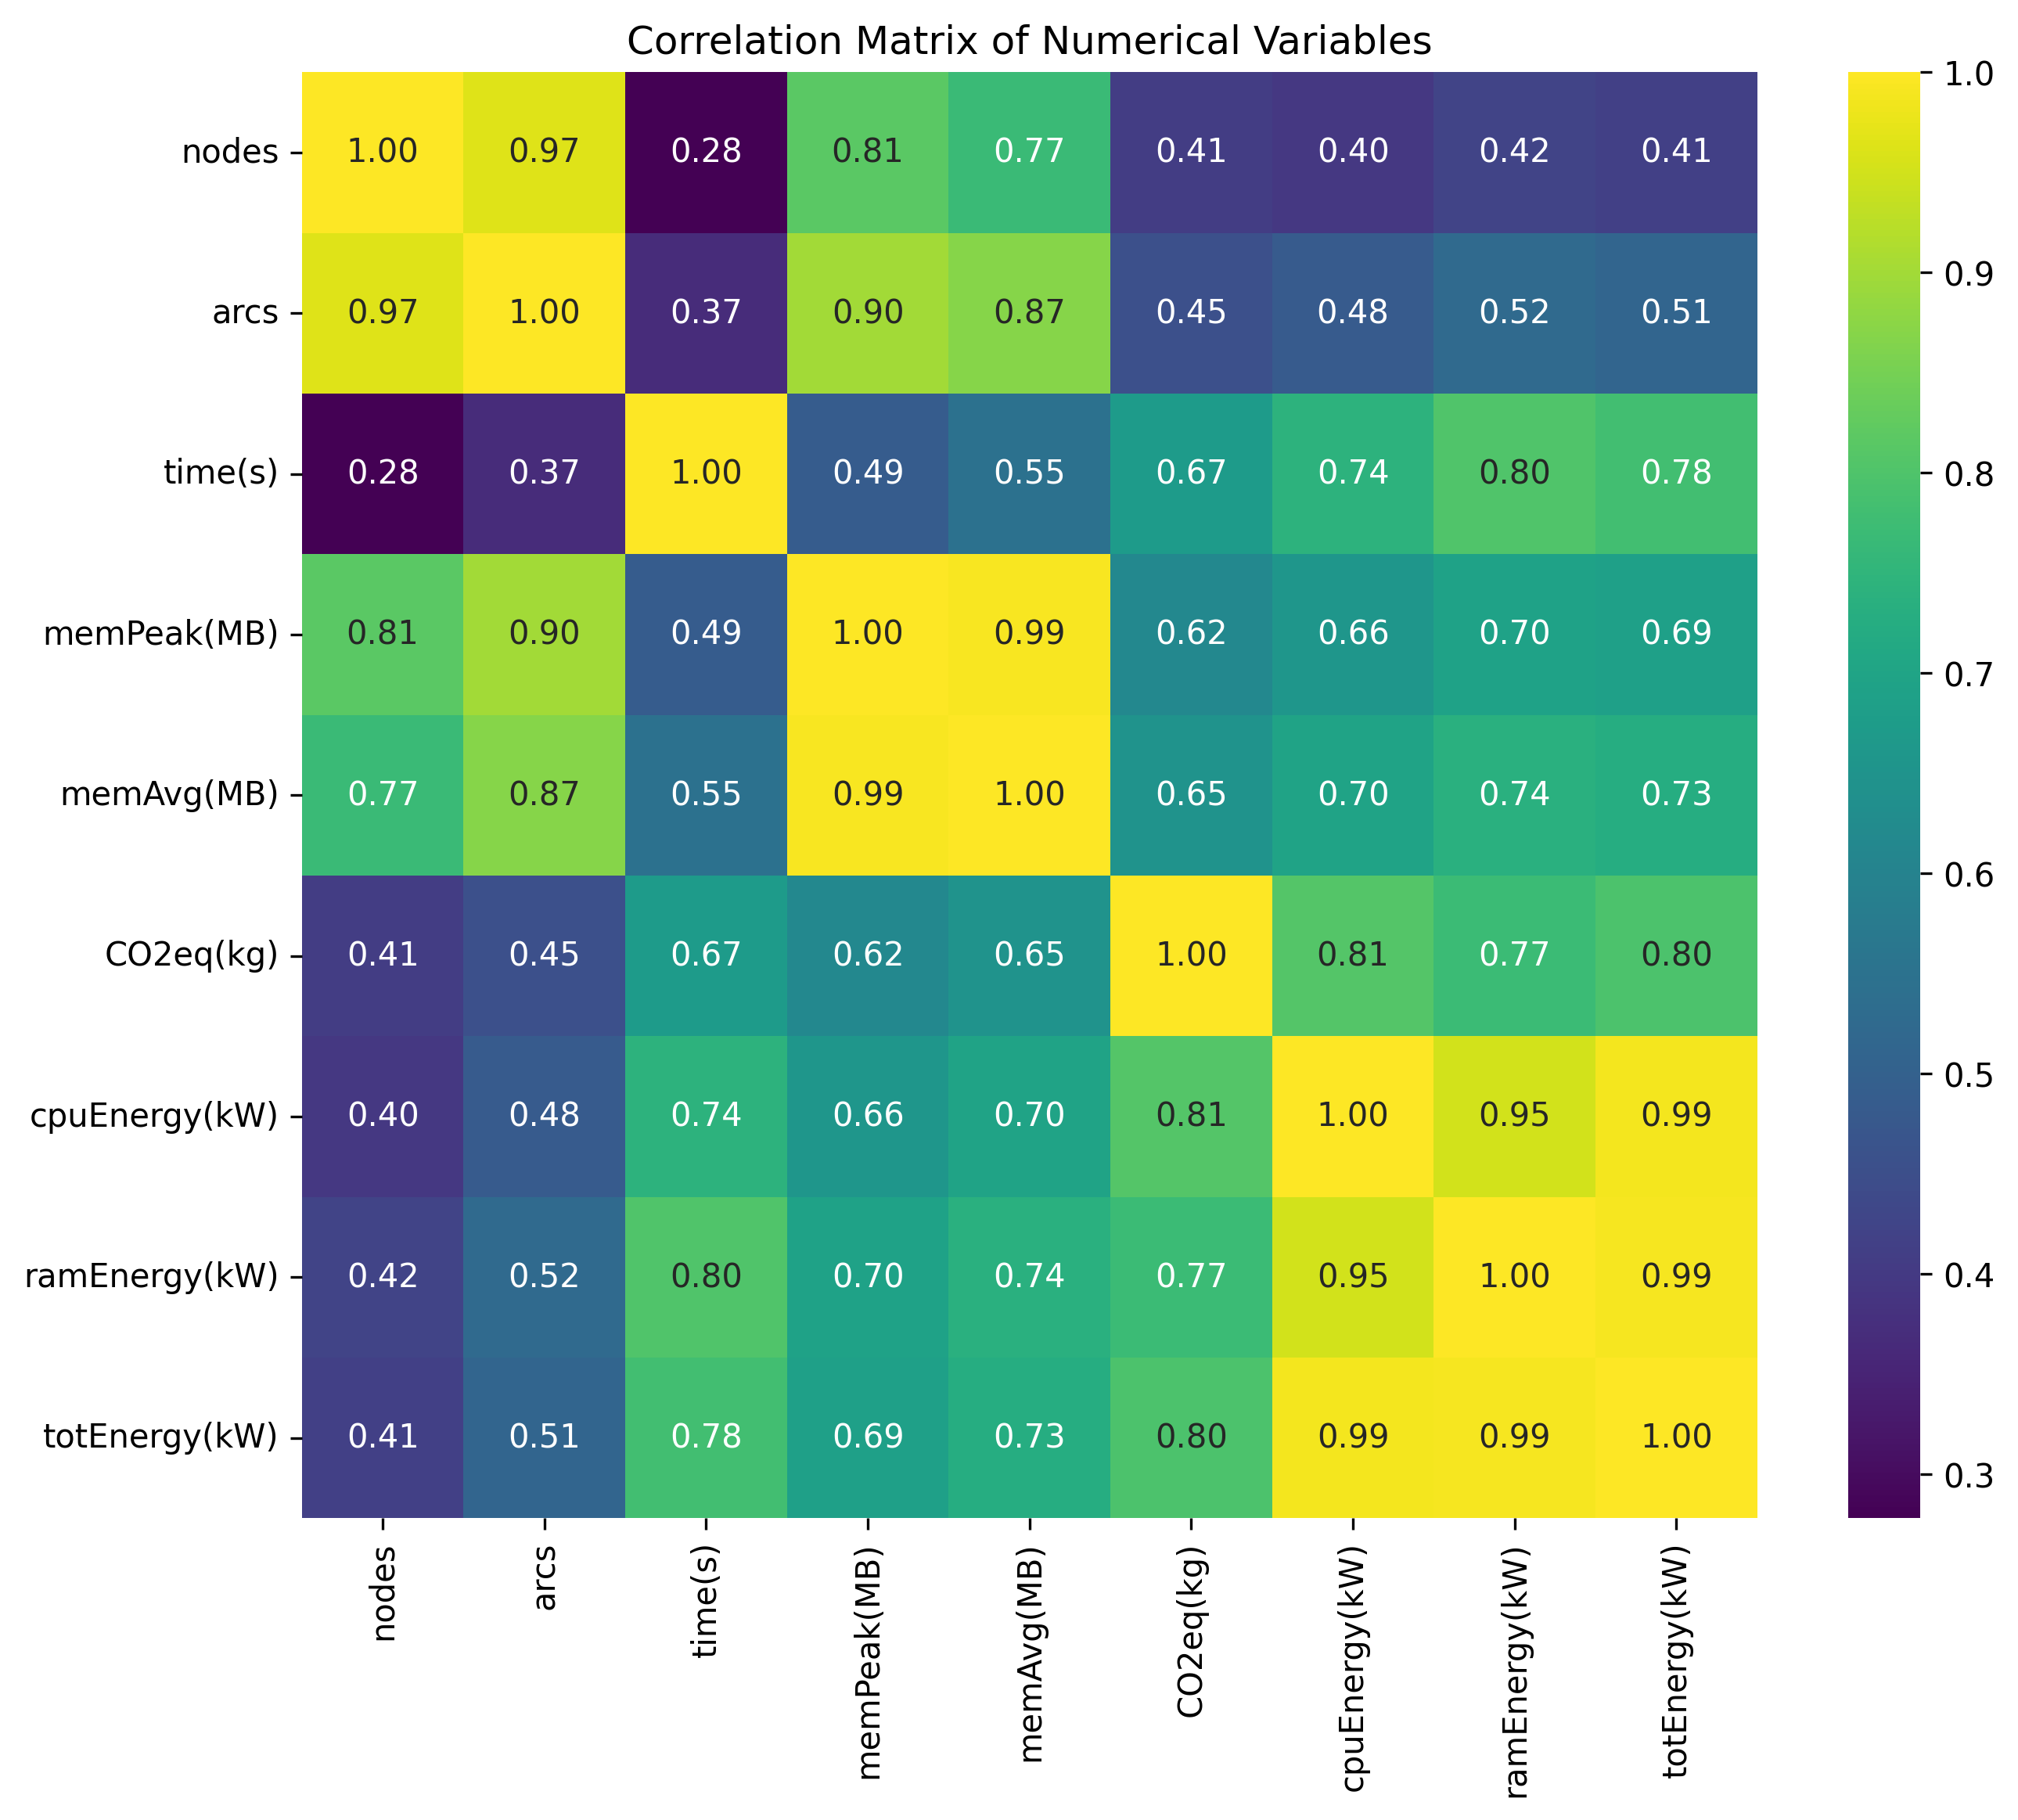
\includegraphics[width=0.8\textwidth]{imgs/max_flow_corr_mat.png}
    \caption{Correlation matrix for Min-Cut/Max-Flow Algorithms BK, EIBFS and HPF}
    \label{fig:max_flow_corr_mat}
\end{figure}

\chapter{HADA-as-a-Service}

\section{HADA Web Application}
Benchmark data was integrated into the HADA web application, requiring:
\begin{itemize}
\item Creation of JSON configuration files for each algorithm-hardware combination.
\item Specification of hyperparameters and performance targets.
\end{itemize}

Example JSON structure:
\begin{verbatim}
{
"name": "anticipate",
"HW_ID": "macbook",
"hyperparams": [
{"ID": "num_scenarios", "type": "int", "LB": 1, "UB": 100}
],
"targets": [
{"ID": "time", "LB": null, "UB": null},
{"ID": "memory", "LB": null, "UB": null},
{"ID": "emissions", "LB": null, "UB": null}
]
}
\end{verbatim}

\chapter{Conclusions}

This work extends HADA by integrating carbon emission constraints, enhancing its applicability 
for sustainable AI hardware selection. Through experimental benchmarks on laptops and HPC systems, 
we validated the framework’s ability to balance performance and environmental impact. The web-based prototype 
enables users to make informed decisions when configuring AI workloads under sustainability constraints.

\appendix

\printbibliography[heading=bibintoc] % biblatex

\acknowledgements
I'm very grateful to the inventor of the Prolog language, without whom this thesis couldn't exist. I'd also like 
to acknowledge my advisor Prof. Mario Rossi by tail-recursively acknowledging my advisor.
	
\end{document}